\documentclass[lettersize,journal]{IEEEtran}
\usepackage{amsmath,amsfonts}
\usepackage{algorithmic}
\usepackage{array}
\usepackage[caption=false,font=normalsize,labelfont=sf,textfont=sf]{subfig}
\usepackage{textcomp}
\usepackage{stfloats}
\usepackage{url}
\usepackage{verbatim}
\usepackage{graphicx}

\usepackage{array}
\usepackage{graphicx}
\usepackage{cite}
\usepackage{subfigure}
\usepackage{amsmath,amssymb,amsthm}
\usepackage[indent,bf]{caption2}
\usepackage{rotating}
\usepackage{setspace}
\usepackage{longtable}
\usepackage{comment}
\usepackage{float}
\usepackage{hyperref}
\usepackage{cleveref}
\usepackage{graphicx}
\newcommand{\crefrangeconjunction}{ to~}
\usepackage{subcaption}
\usepackage{enumitem}
\usepackage{pgfgantt}
%\usepackage{longtable}
 \usepackage{dingbat}
% \usepackage{verbatim}

\usepackage{amsfonts}
\usepackage{amssymb}


%-------------------------------- Defitions
\def \SE {\textbf{SE}(3)}
\def \SO {\textbf{SO}(3)}
\def \se {\textbf{se}(3)}
\def \so {\textbf{so}(3)}
\def \R  {\mathbb{R}}
\def \g  {\mathfrak{g}}

\def \V {\mathcal{V}}
\def  \I {\mathcal{I}}
%\def  \or {\mathcal{o}}
\def  \B {\mathcal{B}}
\def \Ad {\textbf{Ad}}
\def \Add {\mathfrak{Ad}}
\def \L {\mathcal{L}}


\newtheorem{theorem}{Theorem}
\newtheorem{lemma}[theorem]{Lemma}
\renewcommand{\qedsymbol}{$\blacksquare$}
%------------------------------------------


\hyphenation{}
\def\BibTeX{{\rm B\kern-.05em{\sc i\kern-.025em b}\kern-.08em
    T\kern-.1667em\lower.7ex\hbox{E}\kern-.125emX}}
\usepackage{balance}
\begin{document}
\title{Singularity-Free Lagrange-Poincare Equations for Vehicle-Manipulator Systems}
\author{IEEE Publication Technology Department
\thanks{Manuscript created October, 2020; This work was developed by the IEEE Publication Technology Department. This work is distributed under the \LaTeX \ Project Public License (LPPL) ( http://www.latex-project.org/ ) version 1.3. A copy of the LPPL, version 1.3, is included in the base \LaTeX \ documentation of all distributions of \LaTeX \ released 2003/12/01 or later. The opinions expressed here are entirely that of the author. No warranty is expressed or implied. User assumes all risk.}}

\markboth{Journal of \LaTeX\ Class Files,~Vol.~18, No.~9, September~2020}%
{How to Use the IEEEtran \LaTeX \ Templates}

\maketitle

\begin{abstract}
One of the advantages of the developed method is the independence of the forward and differential kinematics maps from the coordinate frame assignment to the intermediate bodies in the multi-body system.


In this paper, we develop a novel singularity-free modelling approach for the dynamics of moving-base space manipulators chasing an non-cooperative target (?in the presence of external disturbing effects) in an orbital environment. We utilize the Lagrange-Poincaŕe (LP) equations by recognizing the independence of the dynamics from the base vehicle's configuration, resulting in a decoupling of the base vehicle's dynamics and the arms motion, reduction of the dynamics.%, that noisy joint acceleration/torque measurements are avoided in the computation of the vehicle motion due to manipulator interaction even while considering external forces.  
The core advantage of the proposed methods is physical con
sistency without level-set assumptions on the momentum map.
We validate this through experiments on both types of OGFM
in the presence of external forces. Finally, the effectiveness of
our approach is validated through a HLS of a fully-actuated

orbital robot while interacting with the environment.
The significance of a proper, geometrically intuitive and powerful mathematical model, Simplicity and computational advantages,
all joints for which the configuration space is a Lie group, such as ball joints and 6-degrees of freedom (dof) “free motion” joints, singularity free,
geometrically viable, all axes in body coordinate frame
including a target and writing everything in base to match with sensing in the base coordinate frame
motion of ee and target is more meaningful in the base frame
ctrl sensing and singularity free in base
We incorporate an extension of the modeling methods for rigid-body mechanisms to be able to model more general joints.
This includes all joints for which the configuration space is a Lie group, such as ball joints and 6-dof “free
motion” joints.
\end{abstract}

\begin{IEEEkeywords}

\end{IEEEkeywords}


\section{Introduction}

\IEEEPARstart{S}{pace} missions, especially those involving handling objects in the Earth's or other planets' orbits, greatly benefit from reliable autonomous robotic systems that are capable of making local decisions.
%Researchers have been investigating robotic means for servicing\cite{meintel1982remote, hinds1982satellite}, refueling, repairing, re-orbiting or retiring satellites in orbit. 
A robot manipulator mounted on a vehicle, called vehicle-manipulator system (also referred to as space manipulator or chaser-manipulator system in this paper) is a compelling universal solution to many in-orbit autonomous operations\cite{Flores-abad2007}. 
(?)Space manipulators provide predictable control over target's behaviour.
These systems are currently used for docking and handling payloads via teleoperation\cite{gibbs2002canada,king2001space, aikenhead1983canadarm}. 
In a space manipulator, the base vehicle has all components of a satellite such as thrusters, Attitude Determination and Control System (ADCS), electronics, telemetry and other subsystems. Its payload is the robotic arm that is deployed once the space manipulator is in the vicinity of a target, in an in-orbit robotic mission.
This article focuses on addressing common problems in the modelling of space-manipulator systems in the manipulator deployment phase. The space manipulator system is mathematically modeled as a multi-body system. The multi-body system consists of a 6 Degree-of-Freedom (DoF) vehicle and a manipulator with a series of joints, most commonly a 3-dof shoulder, a 1-dof elbow, and a 3-dof wrist.
The aim is to analyse the dynamics and enable singularity-free planning and control of the robotic arm from a braked position to reach its end goal. 
The major contributions presented in this article include a complete Lie Group formulation for moving-base multi-body systems with multi-DoF joints and a Lagrange-Poincare formulation of dynamics for a system on a cartesian product of a Lie Group (vehicle configuration) and a shape space (manipulator's internal states), providing a singularity-free representation of the base dynamics and multi-dof joints and effectively decoupling the external and internal dynamics\cite{park1995lie}. We incorporate an extension of the modeling methods for rigid-body mechanisms to be able to model more general joints the single-dof rotary and prismatic ones. 
This includes all joints for which the configuration space is a Lie group, such as ball joints and 6-dof “free
motion” joints. Common dynamic modelling approaches, such as Hamel equations and Lagrange equations, start from the assumption that the configuration space is isomorphic to $\R^n$. Inspired by the “change of basis” technique used in the constrained force algorithm \cite{}(?), a projection operator is incorporated to utilize exponential coordinates (generated by the Lie algebra) as local Euclidean coordinates. The total relative configuration space of two consecutive bodies in the chain can then be covered by an atlas of local exponential coordinate charts (patches?). The dynamics of a system on a single Lie group can be expressed globally in terms of the group and algebra structures. Locally, the dynamics can be expressed in these coordinates, resulting in explicit and
singularity-free differential equations. The main advantages achieved are a reduced number of state variables and elimination of constraint equations (compared to implicit methods); improved numerical stability due to avoiding singularities; and generally easier integration into model-based control methods such as MPC, RL and computed torque by providing explicit differential equations without constraints. 

The paper is structured as follows:


\section{Related Literature}
\label{chap:MainBackground}

The current work focuses on the modeling of a vehicle manipulator in the arm deployment phase of in-orbit robotic missions conducted by a vehicle-manipulator system.
%\subsection{Prior to Deployment of Arm} \label{synch}
%The relative linear and angular motion of the chaser and its target can synchronized in the close-range rendezvous phase and therefore, the multi-body system can have a non-zero total angular momentum during the deployment and autonomous motion control of the robotic arm from a braked position to reach its target.
A vehicle-manipulator system is best represented as a multi-body system consisting of rigid bodies interconnected by ideal joints. It is critical to obtain a simple and yet geometrically meaningful model of the system that is capable of including the distinguishing characteristics of space manipulators. One such characteristic is possessing a freely moving 6-dof base body (vehicle). The consensus among the scientific society is that the ADCS system should be turned off when the end-effector goes into contact with the target to avoid any unexpected response of the control system. Therefore, it is always necessary to plan a free-floating scenario for the robotic system. Many formalisms have been proposed to model multi-body systems, among which screw theory for kinematics\cite{murray2017mathematical} and Hamiltonian/Lagrangian formulation for dynamics\cite{stramigioli2000hamiltonian,Chhabra2014a}{} are particularly advantageous due to their strong geometric roots. Free-floating space robots have un-actuated 6-dof base\cite{Tortopidis}{} introducing challenges for the trajectory planning and control of the system, while on the other hand, enabling the development of energy efficient control strategies\cite{Transactions2013}{} by making use of the internal couplings and the degree of controllability of the system\cite{huang2017path}{}. 
Geometric mechanics is a branch of applied mathematics that studies nonlinear dynamical systems on their configuration manifolds that may or may not exhibit a Lie group structure. The methodology extensively incorporates tools in differential geometry to treat such complex systems in a coordinate-free manner. The configuration manifold includes all possible configurations of the system and the phase space consists of the required states to formulate the dynamics. For example, Lagrangian systems are described by the configurations and their velocities, i.e., elements of the tangent bundle $T\cQ$, and Hamilton's equation are defined based on the configurations and their conjugate momenta, i.e., elements of the cotangent bundle $T^*\cQ$. Therefore, dynamics of a regular system is a vector field on the phase space whose integral curve represents the time evolution of the system\cite{muller2016geometric}. In the case of a rigid vehicle-manipulator system, the configuration manifold of the system is of dimension $n+6$ and it is diffeomorphic to the set of all allowable relative transformations between the rigid bodies forming the system, which exhibits a Lie group structure. 
The idea of reducing the phase space of a nonlinear system and accordingly its associated dynamics, initiated by Marsden and Weinstein\cite{MARSDEN1974} and K. Meyer\cite{meyer1973symmetries}, is at the core of geometric mechanics. Specifically in proximity operations, these free-floating systems are underactuated and non-holonomic due to the existence of an uncatuated base resulting in the conservation of momentum. 
%The property of interest in the trajectory planning of an arm is mainly the absolute angular and linear velocity of the end-effector. 
Trajectory planners have been extensively studied for coupled vehicle-Manipulator systems\cite{Huang2006,Chamitoff2014,King}. Motion of the arm cannot be studied independently of that of the vehicle. Ni et al. propose a shooting method which by varying the speed of the end effector and analyzing it through the theory of calculus of variations generates optimal trajectories\cite{ni2017trajectory}{}.
Rybus and Seweryn investigated the differences between free-floating and free-flying vehicle-arm systems\cite{rybus2018manipulator} and studied trajectory optimization\cite{seweryn2008optimization}, application of Bezier curves for singularity avoidance\cite{Rybus2016}, and capture maneuvers for both cases \cite{rybus2018manipulator}. 
Challenges arise due to non-holonomicity of the arm dynamics such as dynamic singularities\cite{Papadopoulos,Respondek2018} and the need for smooth obstacle avoidance\cite{Papadopoulos2005polynomial,rybus2018obstacle}{}. Importance of Obstacle avoidance and compensating for the contact forces when the end-effector goes into contact with the target? % are critical challenges in planning and control of this system\cite{nagamatsu1996capture}. Researchers minimize the contact reactions, or they design for an end-effector impedance when the chaser-manipulator system is in the final configuration to withstand the contact\cite{Yoshida2015}. A most common approach in dealing with the reaction forces upon impact is by minimizing the impact force via proper choice of the contact point and well-designed pre-impact trajectories. 
A dynamic singularity occurs when the generalized Jacobian matrix\cite{Umetani1989} becomes singular. Tchon, Respondek and Ratajczak addressed this problem by utilizing normal forms of singularities of non-holonomic robots described by control-affine systems\cite{Respondek2018}{}. Robustness and stability of the trajectory following tasks are crucial in in-orbit missions\cite{King,rybus2016trajectory,seddaoui2017optimised}. (ADD??? robust:Boscariol:\cite{boscariol2016optimal}
effect of non-zero momentum (ulrich, DLR) in presence of disturbances
workspace vs joint-space trajectory planning.)
Hussein and Bloch use theory of affine connections along with method of navigation functions and Lagrange multipliers to plan sub-optimal trajectories for a class of underactuated systems with non-holonomic constraints to avoid obstacles\cite{Hussein2008}. They also study constrained optimal trajectory following of a group of rigid bodies with configuration manifolds SE(3) in a finite time\cite{hussein2005constrained}{}. Shammas et al. analyze and generate gaits for mixed mechanical systems whose motion is simultaneously governed by a set of non-holonomic constraints and a conserved generalized momentum. Through proper recourse to geometric mechanics, they are able to show that the resulting motion has two portions: a geometric and a dynamic contribution\cite{pathshammas,pathshammas1}. 
Recently, smart and efficient autonomous navigation techniques based on Riemannian motion policy have been introduced to use in deep learning for vehicle control purposes\cite{Mengnavigation} and demonstrated competent performance in indoor motion control and obstacle avoidance. Adaptive control schemes, due to their ability to adjust themselves according to external and internal changes, are beneficial in dealing with unknown environments and un-cooperative targets. Walker makes use of an adaptive controller to achieve stability despite the uncertainties in the dynamic and inertial parameters of a vehicle-manipulator system\cite{Walker1991}. Wang and Hanlei incorporate a generalized dynamic regressor in adaptive inverse dynamics study of a free-floating vehicle-arm system to account for the nonlinearities due to unknown or varying parameters\cite{Wang2011}. 
Wee et al. demonstrated the capabilities of adaptive control methods in controlling trajectories of a free-floating vehicle and a 6-DOF arm simultaneously by having the adaptive logic acquire parameter estimations through momentum integrals\cite{Wee1997}. %They propose the following adaptive control command to be applied to joint \(i\)\cite{Walker1991}???????????????
%\begin{equation}\tau_i=\sum_{j=1}^m\sum_{k=1}^m Tr[\frac{\partial (^IH_j^I)}{\partialq_i} (\tilde{U}_{jk})(^I\ddot{\tilde{H}}_k^I-\gamma{}^I\dot{\tilde{H}}_k^I)^T]\end{equation}
%With the adaptation law
%\begin{equation}\dot{\tilde{U}}_{jk}=-\alpha_{jk}(^I\dot{\tilde{H}}_k^I)(^I\ddot{\tilde{H}}_k^I-\gamma{}^I\dot{\tilde{H}}_k^I)\end{equation}
%Where \(\gamma\) is a design parameter, \(\alpha\) is a convergence parameter and and \(\tilde{U}_{jk}\) is defined as
%\begin{equation}{}^I\dot{\tilde{H}}_k^I=\sum_{i=1}^k \frac{\partial ^IH_k^I}{\partialq_i}\dot{\tilde{q}}_i\end{equation} 
%With the augmented state error
%\begin{equation}\dot{\tilde{q}}=\dot{q}_d-\lambdaq_e \quad \& \quad \ddot{\tilde{q}}=\ddot{q}_d-\lambda\dot{q}_e\end{equation}??????????????????
Ulrich and Shi demonstrated an adaptive controller's ability to deal with large inertia uncertainties without the need for online estimation\cite{Shi2015}. Ulrich et al. also developed a passivity-based output feedback adaptive control law to improve the stability and robustness of a path-planner for vehicle-arm systems\cite{Ulrich2016}. Less complex adaptive control logics are proven to be effective in controlling space robotic arms despite their simplicity\cite{Ulrich2012}. Ulrich et al. evaluated the performance of a simple adaptive controller\cite{Ulrich2014}{}. 
Adaptive controllers operate on the basis of tuning the control gains based on feedbacks received from the output of dynamical systems. 
\begin{comment}
Ulrich et al. propose a Direct Adaptive Control (DAC) based on an output feedback transpose Jacobian control law \cite{Ulrich2014} (Figure \ref{fig:adaptiveulrich}) for a sample 2-link manipulator:
\begin{equation}\tau_\mathfrak{m} ={}^IJ^I_{ee}(q)^{\textbf{tr}}[K_p(t)e+K_d(t)\dot{e}],\end{equation}
where $e$ is the end-effector position error.  
%the tracking error is
%\begin{equation}e={^IX_{des}^{I}}-{^IX^I_{ee}},\end{equation}
%and \({^IX^I_{ee}}\) is the current pose of the end-effector and \({^IX_{des}^{I}}\) is the desired end-effector pose.
%There are various means by which to generate the controller gains which typically depend on the tracking error in simple adaptive controllers. 
One adaptation logic suggested by Ulrich for their Modified Simple Adaptive Controller (MSAC) is\cite{Ulrich2014}
\begin{equation}K_p=(ee^{\textbf{tr}}\Gamma_{pp})+\int (ee^{\textbf{tr}}\Gamma_{pi}-\delta_pK_{pi}I_{6 \times 6})dt,\end{equation}
and
\begin{equation}K_d=(ee^{\textbf{tr}}\Gamma_{dp})+\int (ee^{\textbf{tr}}\Gamma_{di}-\delta_dK_{di}I_{6\times 6})dt,\end{equation}
where $\Gamma_{pp}$, $\Gamma_{pi}$ , $\Gamma_{dp}$ and $\Gamma_{di}$ are control
parameters adjusted by the designer and $\delta_p$ and $\delta_d$ are small
positive control coefficients used to prevent the integral terms of the control gains from diverging\cite{Ulrich2014}.
% add model predictive: Direct Model Reference Adaptive Control of a Flexible Joint Robot
 Another common adaptive control approach, named Model Reference Adaptive Control (MRAC), includes a reference model and incorporates the output of the model $x_\mathfrak{m}$ along with a scalar reference model input 
signal $\nu_\mathfrak{m}$ in the overall control signal\cite{Ulrich2010a}
\begin{equation}\tau_\mathfrak{m}=\begin{bmatrix}K_e(t) & K_{x_\mathfrak{m}}(t) & K_{\nu_\mathfrak{m}}(t)\end{bmatrix}\begin{bmatrix}e\\x_\mathfrak{m}\\ \nu_\mathfrak{m}\end{bmatrix},\end{equation}
and the control gains are adapted via
\begin{equation}\begin{bmatrix}K_e(t) \\ K_{x_\mathfrak{m}}(t) \\ K_{\nu_\mathfrak{m}}(t)\end{bmatrix}^{\textbf{tr}}=e\begin{bmatrix}e \\ x_\mathfrak{m} \\ \nu_\mathfrak{m}\end{bmatrix}^{\textbf{tr}} \Gamma_p+\int e\begin{bmatrix}e \\ x_\mathfrak{m} \\ \nu_\mathfrak{m}\end{bmatrix}^{\textbf{tr}} \Gamma_{i},\end{equation} 

where $\Gamma_{p}$ and $\Gamma_{i}$ are control parameters, and $K_e(t)$, $K_{x_\mathfrak{m}}(t)$ and $K_{\nu_\mathfrak{m}}(t)$ are gains corresponding to the error, system model output and model input, respectively\cite{Ulrich2010a}.

\end{comment}
Cao and Silva use Neural-Networks to aid their adaptive controller in path-planning for a space robot with flexible joints and links\cite{cao2006dynamic}.
A closed-loop adaptive control requires a sensory system accompanied with a reliable state estimation. 
Ulrich and Sasiadek couple an EKF with an adaptive controller\cite{Ulrich2011a} to develop an adaptive feedback, feed-forward controller for a manipulator with elastic uncertainties at joints\cite{Ulrich2014a}. They demonstrate the adaptation capabilities of a direct adaptive fuzzy control to track the errors between a model and a real space robot\cite{Ulrich2011b}. Sasiadek and Green also apply a fuzzy logic system to adapt the gains of a transpose Jacobian controller in a flexible link robot\cite{Green2005}. 
%%%%%%%%%%%%%%%%%%%%%%%%%%%%%%%%%%%%%%%%
%\subsection{Model-Predictive Adaptive Control Based on Geometric Mechanics} 
Zhenyu Li proposes a self-tuning adaptive control scheme for free-floating space robots with unknown mass properties based on least-square estimation technique\cite{li2016target}. Shibli, Su, and Aghili developed an adaptive controller based on the inverse dynamics of a free-flying space manipulator to perform contact operations\cite{shibli2006adaptive}{}. 
%(Model Predictive Control have a separate section? didn't have enough specific papers to separate adaptive and %model reference, though I should have been able to if I had time) 
Challenges may stem from the uncertainties in the chaser-arm system and its environment, for example, uncertainties in the target model\cite{Abiko}, unaccounted elastic behaviours in the robotic system or the target\cite{Sharf1995,ishijima2005orbit}, and external and internal disturbances\cite{guo2008terminal,Hrobustdevelopment} . Variational-structure control\cite{Wei2011,Saaj2014}{}, robust and adaptabive\cite{Ulrich2015,Ulrich2014a,Sasiadek1988} can address this need.
Therefore, advanced control methodologies capable of handling uncertainties, such as adaptive, robust and sliding mode controllers\cite{saaj2002new,Ulrich2010,Ulrich2014} have been extensively studied in the literature for vehicle-manipulator systems. 

\section{Kinematics of Vehicle-Manipulator Systems on Lie Groups}
\label{math} %\section{Mathematical Background}
%\section{Abstract}
In this section, we provide the kinematic framework that is utilized throughout the article to describe the relative motion of rigid bodies in a moving-base multi-body system based on the Lie Group theory. 


\subsection{Relative Rigid Body Pose and Velocity}
\label{rigidbodykinematics}
%The goal of this section is to provide a formalism for describing motion of a rigid body with respect to a reference coordinate frame or another rigid body. 
Let us consider two rigid bodies in the multi-body system indexed by $i$ and $j$, and attach two orthonormal coordinate frames to them. A relative pose $g^j_i$ between Body $i$ and Body $j$ is a map from the coordinate frame attached to body $i$ to that attached to body $j$ that is isometric and orientation-preserving. The set of all such relative poses forms a smooth manifold that is called the relative configuration manifold and is denoted by $G^j_i$. An element $g^j_i\in G^j_i$ can be represented via %either represented via the pair $(R^j_i,{}^jp^j_i)$ or alternatively via 
\begin{equation}
    g^j_i=\begin{bmatrix}R^j_i & ^jp^j_i\\\boldsymbol{0} &1\end{bmatrix} 
\end{equation}
where ${R^j_i} \in \SO$ is a ${3 \times 3}$ matrix that describes the orientation of the coordinate frame attached to Body $i$ relative to that attached to Body $j$, and $^jp^j_i \in \R^3$ is the vector of relative linear position between the origins of the same coordinate frames expressed in the frame of Body $j$. %Let us denote the space of all coordinate transformations of Body $i$ by $G^i_i \cong \SE$ and Body $j$ by $G^j_j \cong \SE$. 
Fixing a relative pose, say $\bar{g}^j_i$, there exists an identification of $G^j_i$ by the space of coordinate transformations of Body $i$, $G^i_i$, through left translation , i.e. $G^j_i={\bar{g}^j_i}G^i_i$, and one by $G^j_j$ through right translation, i.e. $G^j_i=G^j_j{\bar{g}^j_i}$. The spaces of coordinate transformations $G^i_i$ and $G^j_j$ are both isomorphic to the Special Euclidean group $\SE$, as Lie groups, and their Lie algebras, respectively denoted by $\g_i^i$ and $\g_j^j$, are isomorphic to $\se$ (the Lie algebra of $\SE$). %$G^j_i$ will then be diffeomorphic to the Special Euclidean Group $\SE$.
%--------------------
%\subsubsection{Relative Velocity of Rigid Bodies} 
\label{difkinrigid}
%For two rigid Bodies $j$ and $i$ , the relative motion of one with respect to the other is a smooth curve $g^j_i(t):[t_0,t_f]\rightarrow G^j_i$ on the relative configuration manifold $G^j_i$. 
For a curve $g_i^j(t)\in G_i^j$, the relative velocity of Body $i$ with respect to Body $j$, $\dot{g}^j_i(t)=\frac{d}{dt}g^j_i(t)$, can be observed in the coordinate frame of Body $i$ or Body $j$ via left translation $^i\hat{V}_i^j={g^j_i(t)}^{-1}\dot{g}^j_i(t)\in\mathfrak{g}_i^i$ or right translation $^j\hat{V}_i^j=\dot{g}^j_i(t){g^j_i(t)}^{-1}\in\mathfrak{g}_j^j$, respectively. 
The wedge operator is the vector space isomorphism between $\R^6$ and $\se$, such that,
\begin{equation}
    \hat{V}:=\begin{bmatrix}\tilde{\omega} & v\\0 & 0\end{bmatrix},
\end{equation}
for every $V=[\omega^T\quad v^T]^T\in \R^6$, where $\tilde{\omega}$ is an element of the Lie algebra of $\SO$, denoted by $\so$, and $v \in \R^3$, corresponding to the angular and linear velocities, respectively. The \textit{tilde} operator transforms a vector $\omega\in\R^3$ to a $3 \times 3$ skew-symmetric matrix, such that $\tilde{\omega}p=\omega\times p$, for every $p\in\R^3$. Given the curve $g_i^j(t)$, the two relative velocity matrices are calculated as
%The inverse of the wedge operator is denoted by \textit{vee}. 
\begin{align}
    \begin{split}
   ^i\hat{V}_i^j:&=\begin{bmatrix}({R}^j_i)^T\dot{R}^j_i & (R^j_i)^T{}^j\dot{p}^j_i\\0 & 0\end{bmatrix} \in \g^i_i,\\
    ^j\hat{V}_i^j:&=\begin{bmatrix}\dot{R}^j_i(R^j_i)^T & -\dot{R}^j_i(R^j_i)^T{}^j{p}^j_i+{}^j\dot{p}^j_i\\0 & 0\end{bmatrix} \in \g^j_j.
     \end{split}
     \label{relvel}
\end{align}
%The smooth  manifold $G^j_i$ will then be diffeomorphic to the Special Euclidean Group $\SE$. These two identifications can give rise to two group multiplications on $G^j_i$ that are not necessarily the same, and the fixed pose $\bar{g}^j_i$ acts as the identity element. 
%The rotation part of the coordinate transformation for body $i$ is a member of the Special orthogonal group $R^i_i \in \SO$, and 
%Here, $^iv^i_i$ is a $3 \times 1$ vector belonging to $\R^3$.
%The left and right translation maps by $(g^j_i(t))^{-1}$ are equivalent to left and $L_{g^j_i(t)}$ and right $R_{g^j_i(t)}$ composition maps at point $g^j_i(t)$, respectively. These two representations belong to the Lie algebras $\g^i_i$ and $\g^j_j$.
%Here, $^j\tilde{\omega}^ j_i$ and $^i\tilde{\omega}^ j_i$ are skew-symmetric matrices corresponding to the angular velocity of body $j$ with respect to body $i$ in the coordinate frames attached to body $i$ and body $j$, and the vectors ${}^iv^j_i$ and ${}^jv^j_i$ represent the linear velocity of Body $i$ with respect to Body $j$ expressed in the frames attached to Body $i$ and $j$, respectively.
%Members of the Lie algebra can be identified via a linear mapping between the Lie algebra via the Lie bracket. A Lie Bracket on a matrix lie algebra is defined as the matrix commutator $[A,B]=AB-BA$. This Lie bracket for members of the $so(3)$ lie algebra becomes the cross product $[\tilde{\omega}_1,\tilde{\omega}_2]=\tilde{\omega}_1\times\tilde{\omega}_2$,
%and for a lie algebra isomorphic to $\SE$ takes the form $[(\tilde{\omega}_1,v_1),(\tilde{\omega}_2,v_2)]=(\tilde{\omega}_1\times\tilde{\omega}_2,\tilde{\omega}_1\times v_2-\tilde{\omega}_2\times v_1)$. 
%-----------------------------------
In order to change the coordinate frame of observation, one should use the \textit{Adjoint operator} (for matrix Lie groups):
\begin{equation*}
    ^j\hat{V}_i^j={g^j_i}{}(^i\hat{V}_i^ j)({g^j_i})^{-1}.
\end{equation*}
%of the relative velocities Lie algebra from one coordinate frame to another a conjugate operator is required:
The $6 \times 6$ \textit{Adjoint matrix} which transforms the $\R^6$ representations of the relative velocity vectors from the coordinate frame $i$ to frame $j$ is 
\begin{equation}
    \Ad_{g_i^ j}:=\begin{bmatrix}R_i^ j & (^ j\tilde{p}_i^ j) R_i^ j \\0& R_i^ j\end{bmatrix},
\end{equation}
such that $^j{V}_i^j=\Ad_{g^j_i}{}^i{V}_i^j$. Based on the Lie bracket of the Lie algebras $\g^i_i$ and $\g^j_j$, we can define the \textit{adjoint operator} $\textbf{ad}_{{}^jV^j_i}(\cdot):=[{^jV^j_i},(\cdot)]$,
where in matrix form
\begin{equation}
\textbf{ad}_{{}^jV^j_i}=\begin{bmatrix}^j\tilde{\omega}_i^{j} & 0\\^j\tilde{v}_i^{j} & ^j\tilde{\omega}_i^{j}\end{bmatrix}.
\label{adjlow}
%\textbf{ad}_{{}^j{V}_i^j}
\end{equation}


%%%%%%%%%%%%%%%%%%%
\subsubsection{Joints} \label{joints}
A joint is a mechanism that restricts the relative motion of body $i$ with respect to body $j$.% to a subset of the tangent bundle of the relative configuration manifold $TG^j_i$. 
Here, we exclusively consider 1-degree-of-freedom (dof) joints with the restricted relative configuration manifold $Q_i^j$ (by an abuse of naming convention) correspoding to a single admissible direction of relative velocity, where $Q_i^j$ through left (right) translation maps to a 1-parameter Lie subgroup of $G_i^i$ ($G^j_j$). %Here, we exclusively utilize joints where this subset defines a distribution that corresponds to admissible directions of relative velocity of body $i$ with respect to body $j$ at every relative pose. 
%Let us denote the space of all admissible relative poses of body $i$ with respect to body $j$ considering the joint constraints by $Q^j_i$, and hereinafter call it the relative configuration manifold, by an abuse of naming convention. The dimension of $Q^j_i$ is named the degree-of-freedom (dof) of the joint. 
%The appropriate parameterization of $Q^j_i$ is one of the critical practical problems in mechanics, due to its influence on the efficiency of dynamical analysis and control of multi-body systems. 
%Let us fix $\bar{g}^j_i \in Q^j_i$ and 
%We can define $Q_j$ by the left composition of $Q^j_i$ by the fixed $(\bar{g}^j_i)^{-1}$, then any element in a local neighborhood of $\bar{g}^j_i$ can be parametrized by a local coordinate chart for a neighborhood of the identity element $e_j \in Q_j$. A velocity vector $V^j_i \in T_{g^j_i}Q^j_i$ at an arbitrary relative pose $g^j_i$ can be consequently identified with an element of the induced coordinate chart for the tangent bundle. 
% screw theory
%Chasles' theorem \cite{whittaker1937treatise} states that every rigid body transformation can be achieved by a \textit{screw motion}, %from any initial relative pose $\bar{g}^j_i$, an arbitrary relative configuration $g^j_i \in G^j_i$ of a rigid body can be achieved by a .
%Here, a set of joint parameters called screw joint parameters is introduced. If the relative velocity vector field of two bodies is independent of time, the respective relative motion can be called relative screw motion. The naming stems from an interpretation of  
The exponential map of the Lie group $\SE$ is a diffeomorphism from a local neighborhood of the origin of the Lie algebra $\se$ to a local neighborhood of the identity element of $\SE$, which geometrically corresponds to a simultaneous rotation about and translation along a fixed vector in $\R^3$, where the ratio of translation to rotation is constant.  %, which provides a local coordinate chart to parametrize $Q^j_i$\cite{Chhabra2014a}. %Using the exponential map, the 1-dof revolute, prismatic and helical joints can be (globally) parameterized via 1-dimensional sub-spaces of $\se$ that provide multiple coverings of their configuration manifolds \cite{Chhabra2014}. 
The right (left) translation via a fixed relative configuration $\bar{g}^j_i\in Q_i^j$ along with the group exponential map of $G^j_j$ ($G_i^i$), induced by $\SE$, introduces a parametrization of the relative configuration manifold $Q_i^j$ of 1-dof joints through  
%The screw joint parameters %$q_i \in \R^n$, %physically corresponding to the initial classic joint speeds for a screw motion on the corresponding relative configuration manifold,
%enable the representation of every rigid motion (and by extension a relative configuration $g^j_i$, through left or right translation via a fixed relative configuration) via the group exponential map of an element  as: % that  By incorporating the product of exponentials formula, the transformation matrix $g^j_i\in \SE$ (the action of the group element $g^j_i$ on the point $q_j \in \R $) can be broken into two parts: 
\begin{align}
       g^j_i(q)=\exp(^j\hat{\xi}^j_iq)\bar{g}^j_i=e^{^j\hat{\xi}^j_iq}\bar{g}^j_i,\label{twistform1}\\ g^j_i(q)=\bar{g}^j_i{}\exp(^i\hat{\xi}^j_iq)=\bar{g}^j_i{} e^{^i\hat{\xi}^j_iq} ,
\end{align}
where $q$ is the joint parameter, corresponding to the amount of rotation and/or translation. The \textit{twist vector} $^j\xi_i^j$ ($^i\xi_i^j$) corresponds to the axis of the relative screw motion observed from the coordinate frame of Body $j$ (Body $i$). In this paper, we only work with the right translation map for joint parameterization, i.e., \eqref{twistform1}. The exponential term gives the required transformation to go from the fixed relative configuration $\bar{g}^j_i$ to any relative configuration of the joint. %$\hat{\xi}^i_i$ is called the twist matrix corresponding to screw motion by the $i^{th}$ joint in the system and $q_i$ is the screw joint parameter corresponding to the motion along the allowed DoF of that joint. 
The twist vector and twist matrix for different 1-dof joints can be calculated from the following equations: 
%of $i$th joint in an open-chain multi-body system, defined rigorously in Section \ref{diffkin}, can be geometrically calculated from
\begin{equation}
    ^j\xi^j_i=\begin{bmatrix}^j\varpi_i^j \\^j\nu^j_i\end{bmatrix} \quad \& \quad ^j\hat{\xi}^j_i=\begin{bmatrix}^j\tilde{\varpi}_i^j  & ^j\nu^j_i \\0 & 1\end{bmatrix}, \label{twist1}
\end{equation}
%where, for a 1-DoF joint, $\omega_i^j$ is the axis of rotation of the joint and $^jp^j_i$ is the the position vector of the origin of that joint at the initial configuration. The $4\times4$ matrix representation $\hat{\xi}_i$ belongs to $\SE$ (NO!!! where has this come from??). 
where $^j\varpi_i^j$ represents the axis of rotation of the joint observed from Body $j$, which for prismatic joints becomes zero. For prismatic joints $^j\nu^j_i$ is a unit vector in the direction of translation observed from Body $j$, for revolute joints $^j\nu^j_i= -{}^j\varpi_i^j \times {}^j\rho_i^j$, and for helical joints $^j\nu^j_i= -{}^j\varpi_i^j \times {}^j\rho_i^j+\mathfrak{p}^j_i{}^j\omega^j_i$. Here, $\mathfrak{p}^j_i$ is the pitch of the helical joint, and $^j\rho^j_i$ is the position vector of a point on the joint axis observed from Body $j$, commonly considered to be the position of the joint.
%These two representations of the twist can be transformed into eachother via the \textit{wedge} and \textit{vee} operators
%\begin{equation}
%    {\xi^j_i}^{\wedge}=\hat{\xi}^j_i \quad \& \quad {\hat{\xi}^j_i}^{\vee}=\xi^j_i.
%\end{equation}
The use of Rodrigues' formula provides a means for calculating the exponential term in the parameterization of 1-dof joints \cite{murray1994mathematical}. Let $\hat{\xi}\in\se$ such that $\xi=[\varpi^T\quad \nu^T]^T$:
\begin{equation}
\begin{split}
    e^{\hat{\xi}q}=\begin{bmatrix}I & \nu q \\ 0 & 1\end{bmatrix}, &\quad |\varpi|=0\\
    e^{\hat{\xi}q}=\begin{bmatrix} e^{\tilde{\varpi}q}& (I-e^{\tilde{\varpi}q})(\tilde{\varpi} \time {}v)+\varpi {\varpi}^T \nu q \\0 &1\end{bmatrix}, &\quad |\varpi| = 1
    \end{split}
\end{equation}
where the exponential term $e^{\tilde{\varpi}}=R \in \SO$ corresponds to the rotation part of a transformation, found from Rodrigues' formula ($|\varpi|=1$) \cite{murray1994mathematical}:
\begin{equation}
    e^{\tilde{\varpi}q}=I+\tilde{\varpi}\sin(q)+ \tilde{\varpi}^2\big(1-\cos (q)\big),
\end{equation}
%with $\omega^j_i=^i\omega^j_i$ or $\omega^j_i=^j\omega^j_i$ being the axis of rotation of the joint.
%expand $ e^{\hat{\omega}^j_iq_i}$.
and the term $(I-e^{\hat{\varpi}q})(\varpi \time {}\nu)+\varpi {\varpi}^T \nu q$ represents the linear translation. 

\subsection{Moving-Base Manipulator System Kinematics}\label{kinematics}
A vehicle-manipulator system moving with respect to an inertial frame $\mathcal{I}$ can be modelled as an open-chain multi-body system. An open-chain multi-body system is a collection of $n$ bodies and $n-1$ joints between the bodies. The coordinate frame of the base vehicle $\B$ is indexed $0$. To avoid complexity in notation, we only study a single-branch arm. The extension of this work to multi-branch manipulators is straightforward. It is advantageous to attach reference frames to each link at the joints and to express the quantities associated with each link in terms of these local frames. The manipulator links are indexed by the set $\{1,\cdots,n\}$, where $n$ corresponds to the end-effector and is interchangeably referred to as $ee$.
Let $Q^I_0$ denote the relative configuration manifold of the base vehicle with respect to the inertial frame $\mathcal{I}$, which, in this study. As specified in Section \ref{joints}, the relative configuration manifold $Q^{I}_0$ is identified via a Lie group through the left translation by a fixed relative pose $\bar{g}^I_0{} \in Q_0^I$. The developed formulation of this article is applicable to any moving-base manipulator system where the motion of the base can be identified via a Lie Group (e.g. planar motion, ball joint, rail, or $\SE$ as in drones, aircraft and vehicles). We have chosen the initial relative configuration in a robotic operation as the aforementioned fixed pose $\bar{g}^I_0{}$. To avoid singularities due to parameterization, we will directly work with members of $Q^I_0$ when formulating the kinematics and dynamics of the system. %This treatment of the base configuration avoids all forms of kinematic singularities in their entirety.  %(?) $D^o_b$ and $D^I_b$ are therefore 6-DoF spaces. 
The relative configuration manifolds $Q^{i-1}_i $ $(i=1, \cdots, n) $ of consecutive manipulator links, on the other hand, are parameterized using the exponential map: $$g_i^{i-1}=\exp{({}^{i-1}\hat{\xi}^{i-1}_iq_i)}\bar{g}^{i-1}_i\in Q_i^{i-1}$$ where ${}^{i-1}\hat{\xi}^{i-1}_i$ is the joint axis defined in \eqref{twist1}, $q_i$ is the joint parameter, and $\bar{g}^{i-1}_i$ belongs to $Q^{i-1}_i$. Here, we only consider one-parameter sub-groups of $\SE$ to describe the relative configuration manifolds of the manipulator joints, which correspond to 1-dof rotary, prismatic and helical joints. %Therefore, an exponential formulation of robot joint motion is utilized to form the relative position  of each manipulator body $i$ with respect to its preceding body in the chain $j$ based on the joint parameter $q_i$. %The manipulator joints are modeled as 1-DoF rotary and prismatic joints. so their $D_i^j$ is a 1-DoF space. 
Let $Q_\mathfrak{m}$ denote the $n$-dimensional configuration manifold of the manipulator. An element $q_\mathfrak{m} \in Q_\mathfrak{m}$ consists of a set of joint parameters of the manipulator $[q_1,\cdots,q_n]^T$. Let $Q$ denote the $n+6$-dimensional configuration manifold of the space manipulator. An element $q \in Q$ consists of a set of velocities of the base vehicle and joint parameters of the manipulator.%The configuration manifold $Q_\mathfrak{m}$ includes all possible values of the joint parameters.
\subsubsection{Forward Kinematics}
\label{forwardkinematics}
%A configuration of the moving-base open-chain multi-body system is defined as the collection of relative configurations of the individual bodies $q:=(g^I_0 ,q_\mathfrak{m}) \in Q^I_0 \times Q_\mathfrak{m}$.
Given a base configuration $g^I_0 \in Q_0^I$, and a set of joint angles $q_\mathfrak{m} \in Q_\mathfrak{m}$,  % and the geometry of the vehicle, arm and the orbits, 
the \textit{Forward Kinematics} (FK) is a smooth map from $q:=(g^I_0 ,q_\mathfrak{m}) \in Q^I_0 \times Q_\mathfrak{m}$ to the pose of one of the bodies in the chain with respect to a chosen frame. For the purposes of this section, this reference frame can be the base vehicle's or the inertial frame.
The configuration of the end-effector with respect to the inertial frame is formed by concatanating the individual rigid motions
\begin{equation}
    g^I_{n}=g^I_{0}g^0_1(q_1)...g^{n-1}_{n}(q_{n}).
\end{equation}
The base vehicle's configuration 
%\begin{equation}
%    g^I_o(q_o)=e^{\hat{\xi}_{o_\theta}q_{o_\theta}}e^{\hat{\xi}_{o_r}q_{o_r}}g^I_o(0)
%\end{equation}
\begin{equation}
    g^I_0 =\begin{bmatrix}R^I_0 & ^Ip^I_0\\0&1\end{bmatrix}
\end{equation}
results directly from it's rigid body dynamics. For simplicity, $^Ip^I_0$ and $R^I_0$ are the position of the center of mass of the base vehicle and its orientation with respect to the inertial frame expressed in the same frame. %The generalized exponential formula for the Forward Kinematics map corresponding to the manipulator can be formulated as
The configuration of each of the bodies in the manipulator can be calculated with respect to the vehicle frame and the inertial frame, and represented in the same frames respectively via the use of generalized exponential formula:
\begin{equation}
    g^0_i(q_\mathfrak{m})=e^{\hat{\xi}_{1}q_{1}}...e^{\hat{\xi}_{i}q_{i}}\bar{g}^0_{i},
\end{equation}
\begin{equation}
    g^I_i(g^I_0, q_\mathfrak{m})=g^I_0e^{\hat{\xi}_{1}q_{1}}...e^{\hat{\xi}_{i}q_{i}}\bar{g}^0_{i},
\end{equation}
were $\bar{g}^0_i$ is a fixed relative configuration of Body $i$ with respect to the vehicle (commonly chosen to be the initial configuration), and the new notation $\hat{\xi}_i={}^{\bar{0}}\hat{\xi}^{i-1}_i$ represent the manipulator joint twist matrices in the multi-body chain, calculated rigorously in Section \ref{diffkin}:
\begin{equation}
    ^{\bar{0}}\hat{V}^{i-1}_i=\big(\Ad_{\bar{g}^0_{i-1}}{}^{i-1}\hat{V}_{i}^{i-1}\big)=^{\bar{0}}\hat{\xi}^{i-1}_i\dot{q}_i=\hat{\xi}_i\dot{q}_i
    \label{twist}
\end{equation}
In order to calculate the kinetic energy, we need to find the pose of the centers of mass of the bodies instead of their coordinate frames:
\begin{equation}
    g^I_{cm,i}=g^I_0e^{\hat{\xi}_{1}q_{1}}...e^{\hat{\xi}_{i}q_{i}}g^i_{cm,i}\bar{g}^0_{cm,i}
\end{equation}


\subsubsection{Differential Kinematics} \label{diffkin}
\begin{lemma}
In matrix form the velocity of Body $i$ relative to the inertial frame can be represented in the frame of inertia or Body $i$ as
\begin{equation}
{}^IV_i^I(q)= {}^IJ^I_i\begin{bmatrix}^0V^I_0\\\dot{q}_\mathfrak{m}\end{bmatrix} \quad \& \quad ^iV_i^I(q)={}^iJ^I_i\begin{bmatrix}^0V^I_0\\\dot{q}_\mathfrak{m}\end{bmatrix}. \label{bodyvelocity}
\end{equation}
where the inertial and body jacobian matrices are
\begin{equation}
    ^IJ^I_i(q)=\Ad_{g^I_0} {}^0J^I_i \quad \& \quad {}^iJ^I_i(q)=\Ad_{(g^0_i)^{-1}}{}{}^0J^I_i,
    \label{bodyjacobian}
\end{equation}
and the base jacobian matrix is
\begin{equation}
    ^0J^I_i(q)=\begin{bmatrix} I  & \hat{\xi}_{1}\cdots \Ad_{e^{\hat{\xi}_{1}q_{1}}\cdots e^{\hat{\xi}_{i-1}q_{i-1}}}\hat{\xi}_i & 0\cdots 0\end{bmatrix},
    \label{basejacobian}
\end{equation}
where the twist $\hat{\xi}_i$ has been rigorously defined by \eqref{twist}.
\end{lemma}
\begin{proof}[Proof ] In an open-chain multi-body system, there exists a unique path between the inertial frame and each body in the chain. The velocity of each Body $i$ in the multi-body system relative to the inertial frame is found by adding up all the relative velocities of neighbouring bodies in that path starting from the base's velocity relative to the inertial frame all the way up to the velocity of Body $i$ relative to Body $i-1$:
\begin{equation}
    ^IV^I_i={}^IV_{0}^I+{}^IV_{1}^{0}+\cdots+{}^IV_{i}^{i-1}, \label{eqinertialvel}
\end{equation}
where all the individual relative velocities must belong to a common Lie algebra $g^I_I$.
The formulation of rigid Body velocity as presented in Section \ref{difkinrigid} \eqref{relvel} provides the velocity of each Body $j$ in a multi-body chain with respect to its neighbour Body $j-1$, represented in either the neighbor body frame $j-1$ or the body frame $j$. In order to add several velocities $^{j-1}V^{j-1}_j$ which individually belong to $\g^I_I$, $\g^b_b$, ... and $\g^{i-1}_{i-1}$, we should map all of these velocities to one common frame $I$.
It can be seen from \ref{difkinrigid} \eqref{adjoint} that $\forall i\in\{b,1,\cdots,n\}$ the velocity of each Body $i$ in the space manipulator relative to its neighbouring Body $i-1$ expressed in the inertial frame is calculated from 
\begin{equation}
    {}^{I}V_i^{i-1}=\Ad_{g^{I}_0 g_{i-1}^0}{}^{i-1}V_i^{i-1}.
\end{equation}
Using this property, the inertial velocity in \eqref{eqinertialvel} can be reformed as
\begin{equation}
    {}^IV^I_i={}^IV_{0}^I+\Ad_{g^I_0}{}^0V_{1}^{0}+\Ad_{g^I_0g^0_1}{}^1V_{2}^{1}+\\
    \cdots+\Ad_{g^I_0g^0_{i-1}}{}^{i-1}V_{i}^{i-1}
\end{equation}
The base's velocity can be identified via a left translation by $g^I_0$ to the Lie algebra of the base
\begin{equation}
    ^0\hat{V}_0^I=({g_0^I})^{-1}\dot{g}_0^I \in \g^0_0.
\end{equation}
If the base vehicle is modeled as 6-dof rigid body, its velocity, belonging to $\g^0_0$, is parameterized by angular velocity $^0\omega^I_0$ and linear velocity $^0v^I_0$:
\begin{equation}
    ^0\hat{V}_0^I=\begin{bmatrix}{}^0\tilde{\omega}_0^I&^0v^I_0\\0 & 0\end{bmatrix} \in \g^0_0
\end{equation}
It is worth noting that quasi-velocities are used to parameterize the velocity space Lie algebra $\g^0_0$ of the vehicle, meaning that these velocities are not direct derivatives of the quantities that describe the configuration spaces (not parameterized in this study). 
\begin{comment}
This means
\begin{equation}
^ bV_b^ o=\begin{bmatrix}^bv^o_b\\\omega^ o_b\end{bmatrix}=\begin{bmatrix} -\dot{R}^ o_bR^b_ o{p}^ o_b+\dot{p}^ o_b\\(\dot{R}^ o_b{R}^b_ o)^\vee\end{bmatrix},
\end{equation}
and in orbital frames
\begin{equation}
    ^oV_b^ o=\begin{bmatrix}^ov^ o_b\\^o\omega^ o_b\end{bmatrix}=\begin{bmatrix}R_b^ o & (^ o\tilde{p}_b^ o) R_b^ o \\0& R_b^ o\end{bmatrix}{}^bV_b^ o
\end{equation}

\end{comment}
Next, the configuration of each body in the manipulator chain $g^{i-1}_i$ has been parameterized by screw joint parameters:
\begin{multline} {}^IV^I_i={}^IV_0^I+\Ad_{g^I_0}{}^0V_{1}^{0}+\Ad_{g^I_0e^{\hat{\xi}_1q_1}}\big(\Ad_{\bar{g}^0_1}{}^1V_{2}^{1}\big)+\\
    \cdots+\Ad_{g^I0e^{\hat{\xi}_1q_1}\cdots e^{\hat{\xi}_{i-1}q_{i-1}}}\big(\underbrace{\Ad_{\bar{g}^0_{i-1}}{}^{i-1}V_{i}^{i-1}}_\text{twist definition root}\big).
\end{multline}
Thus, the velocity of Body $i$ in the chain with respect to the inertial frame represented in the inertial frame can be simplified to:
\begin{equation}
    {}^IV_i^I(q)={}^IV_0^ I+\Ad_{g^{I}_0}{}\xi_1\dot{q}_1+\cdots+\Ad_{g^{I}_0e^{\hat{\xi}_{1}q_{1}}\cdots e^{\hat{\xi}_{i-1}q_{i-1}}}\xi_i\dot{q}_i.
\end{equation}
Considering the fact that a space manipulator's planning and control system works within the frame of the base vehicle, the space manipulator's contribution to the velocity of Body $i$ relative to the inertial frame is represented in the frame of the base vehicle:
\begin{equation}
    ^IV_i^{I    }(q)={}^IV^I_0(t)+\Ad_{g^I_0}{}^0V^I_i(q),
\end{equation}
where
\begin{equation}
    ^0V^I_i=\xi_1\dot{q}_1+\cdots+\Ad_{e^{\xi_{1}q_{1}}\cdots e^{\xi_{i-1}q_{i-1}}}\xi_i\dot{q}_i,
\end{equation}
providing the motivation for the definition of jacobian in Equations \ref{bodyjacobian} and \ref{basejacobian}, and derivation of \eqref{bodyvelocity}.
\end{proof}
Since these velocities will be paired with body inertia matrices in calculating the kinetic energy, we have represened the velocity of each body relative to the inertial frame in the body coordinate frame too. %Therefore, the body Jacobian is presented:
% as a result we can say
% \begin{multline}
%     {}^iJ^o_i(q)=Ad_{(g^b_i)^{-1}}{}\begin{bmatrix} I_{6\times 6}  & \xi_{1}\cdots Ad_{e^{\xi_{1}q_{1}}\cdots e^{\xi_{i-1}q_{i-1}}}\xi_i & 0\cdots 0\end{bmatrix}\\
%     =\begin{bmatrix}Ad_{g^b_i(0)^{-1}e^{-\xi_{i}q_{i}}\cdots e^{-\xi_1q_1}}I_{6 \times 6} & Ad_{g^b_i(0)^{-1}e^{-\xi_{i}q_{i}}\cdots e^{-\xi_1q_1}}\xi_{1}& \cdots &Ad_{ g^b_i(0)^{-1}e^{-\xi_iq_i}}\xi_i & 0& \cdots& 0\end{bmatrix} 
%     \label{bodyjacobian}
% \end{multline}
It is worth pointing out here the fact that the body velocity $^iV^I_i$ turned out to be completely independant of $\Ad_{g^I_0}$, which translates to the dynamics of the system being symmetric with respect to the configuration of the base body. This means that the dynamics of the system has the same shape and characteristics any configuration of the base vehicle. 

%\subsection{Case Study?}

\begin{comment}



\begin{figure}[htbp]
\begin{center}
\begin{tikzpicture}[x=1cm, y=1cm, z=-0.6cm, scale=0.7]
    % Axes
    \draw [->] (-2.5,-1.5,0) -- (-1.5,-1.5,0) node [at end, right] {$z$};
    \draw [->] (-2.5,-1.5,0) -- (-2.5,-0.5,0) node [at end, left] {$x$};
    \draw [->] (-2.5,-1.5,0) -- (-2.5,-1.5,1) node [at end, left] {$y$};
    
    
    
    % bodies
    %\draw[fill=gray!50] (0,0,2) circle (0.4); 
    \draw[black, very thick, fill=gray, rotate around={0:(1.3,0.4)}] (0,0) circle (1.5) ;
    \draw[black, very thick, fill=white, rotate around={40:(1.3,0.4)}] (2.5,0) ellipse (1.5 and 0.5);
    \draw[black, very thick, fill=white, rotate around={-30:(1.3,0.4)}] (3,0) ellipse (1.5 and 0.5);
    \draw[black, very thick, fill=white, rotate around={30:(1.3,0.4)}] (3.7,-2.5) ellipse (1.5 and 0.5);
    % \draw[black, very thick, fill=white, rotate around={65:(3.5,1.5)}] (4.8,1.8) ellipse (1.5 and 0.5);
    \draw[black, very thick, fill=white, rotate around={15:(4,1.4)}] (4.6,1.8) ellipse (1.5 and 0.5);

 
    \filldraw[black] (6.6,2.1) circle (1.5pt); \filldraw[black] (7,1.9) circle (1.5pt); \filldraw[black] (7.4,1.7) circle (1.5pt);
 
    \draw[black, very thick, fill=white, , rotate around={-35:(9,2)}] (9.8,0.7) ellipse (1.5 and 0.5);
 
    
    
    % Labels
    \node [left] at (0.5,2.4,1) {$B_b$};
    \node [right] at (1,1.4,0) {$B_1$};
    \node [right] at (3.8,2.9,0) {$B_2$};
    \node [right] at (9,1.2,0){$B_n$};
    \node [right] at (5.65,-1.2,0){$B_{1'}$};
    \node [right] at (1.35,-1.4,0){$B_{2'}$};
    
    % Axes 1
    \draw [->, rotate around={0:(1.3,0.4)}] (-1.5,0,0) -- (-0.5,0,0) node [at end, right] {$z_b$};
    \draw [->, rotate around={0:(1.3,0.4)}] (-1.5,0,0) -- (-1.5,1,0) node [at end, left] {$x_b$};
    \draw [->, rotate around={0:(1.3,0.4)}] (-1.5,0,0) -- (-1.5,0,1) node [at end, left] {$y_b$};
    
    % Axes 2
    \draw [->, rotate around={40:(1.3,0.4)}] (1,0,0) -- (2,0,0) node [at end, right] {$z_1$};
    \draw [->, rotate around={40:(1.3,0.4)}] (1,0,0) -- (1,1,0) node [at end, right] {$x_1$};
    \draw [->, rotate around={40:(1.3,0.4)}] (1,0,0) -- (1,0,1) node [at end, left] {$y_1$};
    
    % Axes 3
    \draw [->, rotate around={15:(4,1.4)}] (3.3,1.7,0) -- (4.3,1.7,0) node [at end, right] {$z_2$};
    \draw [->, rotate around={15:(4,1.4)}] (3.3,1.7,0) -- (3.3,2.7,0) node [at end, left] {$x_2$};
    \draw [->, rotate around={15:(4,1.4)}] (3.3,1.7,0) -- (4.2,1.7,1) node [at end, right] {$y_2$};
    
    % Axes m
    \draw [->, rotate around={-35:(9,2)}] (8.3,0.7,0) -- (9.3,0.7,0) node [at end, right] {$z_n$};
    \draw [->, rotate around={-35:(9,2)}] (8.3,0.7,0) -- (8.3,1.7,0) node [at end, left] {$x_n$};
    \draw [->, rotate around={-35:(9,2)}] (8.3,0.7,0) -- (8.3,0.7,1) node [at end, left] {$y_n$};
    
    % Axes 3'
    \draw [->, rotate around={30:(1.3,0.4)}] (2.35,-2.5,0) -- (3.35,-2.5,0) node [at end, right] {$z_2'$};
    \draw [->, rotate around={30:(1.3,0.4)}] (2.35,-2.5,0) -- (2.35,-1.5,0) node [at end, left] {$x_2'$};
    \draw [->, rotate around={30:(1.3,0.4)}] (2.35,-2.5,0) -- (2.35,-2.5,1) node [at end, left] {$y_2'$};

\end{tikzpicture}
\end{center}
\caption{A general vehicle-manipulator system with general shape and properties, modeled as $m$ open chains each of $n^m$ bodies}
\label{multibody}
 
\end{figure}
Imagine a manipulator mounted on a vehicle which is moving relative to an inertial frame with an absolute configuration of
\begin{equation}
    g^I_0=\begin{bmatrix}R^I_0 & {}^Ip^I_0\\0 & 1\end{bmatrix} \in Q^I_0 \cong \SE
\end{equation}
The most common space manipulator, a shoulder-elbow-wrist, includes two ball joints. We choose the configuration matrix Q to be the 3 × 3 rotation
matrix that describes the relative orientation of frames Ψ1 and
Ψ2, such that their relative configuration satisfies We can choose the coordinate mapping Ψ using exponential
coordinates, i.e., as
\begin{equation}
    g^0_1=\begin{bmatrix}R^0_1 & 0\\0 & 1\end{bmatrix} \in \R^{4 \times 4}
\end{equation}
\begin{equation}
    g^2_3=\begin{bmatrix}R^2_3 & 0\\0 & x1\end{bmatrix} \in \R^{4 \times 4}
\end{equation}
As the global velocity coordinates, we pick v ∈ R3 to be the
angular velocity vector of frame Ψ2 relative to Ψ1, expressed in
Ψ1. The relative twist between Ψ1 and Ψ2 then becomes
\begin{equation}
    I_{3 \times 3} \\
    0_{3 \times 3} 
\end{equation}
we can choose the coordinate mapping Ψ using exponential
coordinates, i.e., as
\begin{equation}
    \Phi(Q,\phi)=Q\textbf{exp}(\tilde{\phi})
\end{equation}
with $\tilde{Phi} = (\Phi∧)$. Rodrigues’ formula \ref{rodrigues} provides an explicit expression for this infinite series.

\subsection{Holonomic Joints}
A globally parameterized holonomic joint is a smooth
$k$-dimensional submanifold $Q \cong SE(3)$ that describes the permitted relative configurations Hi j of body j relative to body i, and satisfies the following properties.
Every joint configuration is uniquely described by a coordinate
matrix Q (of arbitrary but constant dimensions),
and Hi
j = Hi
j (Q). We identify an abstract element of Q
with its coordinate representation Q and write Q ∈ Q.
2) Every allowed joint velocity (an element of the tangent
space TQQatQ) is uniquely described by a vector v ∈ Rk ,
and the joint twist can be expressed as Ti,i
j = X(Q)v with
X(Q) ∈ R6×k a matrix describing the instantaneously allowed
twists.
3) There exists a coordinate mapping Φ : Q×Rk →Q,
such that for each Q ∈ Q, Φ(Q, 0) = Q and Φ(Q, ·) defines
a local diffeomorphism between a neighborhood of
0 ∈ Rk and a neighborhood of Q ∈ Q. Every point of the allowed
configuration space is assigned a unique coordinate Q, and the mapping Φ maps local Euclidean coordinates ϕ to a
neighborhood of every Q. Although the requirement for the mapping Φ may seem restrictive,
the class of joints that satisfy Definition 1 is actually
quite large. First, classical joints with a Euclidean configuration
space can be formulated in the form of the definition. For a
joint with k degrees of freedom, the global configuration coordinate
can be chosen as Q ∈ Rk , its velocity coordinate as
v = ˙Q ∈ Rk , and the coordinate mapping as Φ(Q, ϕ) = Q + ϕ
with ϕ ∈ Rk . Second, joints with a configuration space described by a Lie
group (e.g., ball joints or “free motion” joints) can also be formulated
as in Definition 1. In this case, the coordinate matrix
Q is the appropriate matrix representation of the Lie group and
the velocity coordinates are the coordinates for the algebra of
the group. The coordinate mapping Φ can be chosen as the
exponential coordinate mapping of the group, i.e., the mapping. with bi the appropriate basis elements for the algebra. Indeed,
Φ(Q, 0) = Qe0 = Q and the mapping maps local coordinates
ϕ to a neighborhood of every Q ∈ Q.

\end{comment}


%\subsection{forces and wrenches?}
%%%%%%%%%%%%%%%%%%%%%%%%%%%%%%%%%%%%%%%%%%%%%%%%%%%%%%%%%%
%%%%%%%%%%%%%%%%%%%%%%%%%%%%%%%%%%%%%%%%%%%%%%%%%%%%%%%%%%
%%%%%%%%%%%%%%%%%%%%%%%%%%%%%%%%%%%%%%%%%%%%%%%%%%%%%%%%%%
%%%%%%%%%%%%%%%%%%%%%%%%%%%%%%%%%%%%%%%%%%%%%%%%%%%%%%%%%%

\section{Vehicle-Manipulator System Dynamics}
\label{chap:Dynamics}
The moving-base multi-body robot's dynamics include the coupled motion of the robotic arm and the base vehicle. The Euler-Poincare formula can provide the dynamics of a decoupled rigid base intrinsically independent of the system configuration's parametrization. Euler-Poincaré equations can be viewed as the reduction of the Euler-Lagrange equations from the tangent bundle of a Lie group to its Lie algebra. In this section, we present an intrinsic (coordinate-free and therefore, singularity-free) and geometric way of writing the reduced dynamic equations on a cartesian product of a Lie Group (moving base) and a shape space (manipulator), called the Lagrange–Poincare equations. The reduced equations are a combination of standard Euler-Lagrange equations for the parametrized portion of the configuration space (arm motion) $T Q/Q^I_0=TQ_\mathfrak{m}$ and Euler-Poincaré equations for the Lie group portion (base) $Q^I_0$. This allows for a nice decomposition between the singularity-free dynamics of the base and the manipulator dynamics. Any disturbance that can be further added is also easily decoupled between the two in this formulation. %(?? A key point in doing this is to decompose the variations of curves in $Q$ into vertical and horizontal components.)
%\section{Lagrange-Poincare Formulation of Multi-Body System Dynamics}
%Dynamics Formulation on a Cartesian Product of a Lie Group and a Shape Space?

\begin{theorem} Given a moving-base multi-body system with base configuration $g^I_0$, arm coordinates $q_\mathfrak{m}$, body velocities ${}^iV^I_i$, arm input $F_\mathfrak{m}$ and total input $F_\Omega$, individual body masses ${}^i\mathcal{M}_i$, overall angular momentum $P$, and kinetic energy $K=\sum \frac{1}{2} {{}^iV_i^I}^T(^i\mathcal{M}_i){}^iV_i^I$, the decoupled external and internal dynamics can be written as
\begin{align}
    -\dot{P}+\textbf{ad}^*_{^0V^I_0}P=F_{\Omega}
    \label{euler-poincare_eq}
\end{align}
\begin{equation}
    {\hat{M}_{m}\ddot{q}_\mathfrak{m}+\dot{q}_\mathfrak{m}^T\hat{C}_{m}\dot{q}_\mathfrak{m}+\hat{N}_{m}=F_\mathfrak{m}-F_{\Omega}J_{sp},}
\end{equation}
with
\begin{equation}
    P=\frac{\partial l}{\partial \Omega}=M_0 \Omega + M_0 J_{sp}\dot{q}_\mathfrak{m},
\end{equation}
\begin{equation}
    \hat{M}_\mathfrak{m}=M_\mathfrak{m}-J_{sp}^TM_0J_{sp},
\end{equation}
\begin{equation}
    {(\hat{C}_{m})=\bigg(\sum\frac{\partial \hat{M}_\mathfrak{m}}{\partial{q}_i}\dot{q}_i-\frac{1}{2}\begin{bmatrix}\dot{q}^T\frac{\partial \hat{M}_\mathfrak{m}}{\partial q_1}\\\dot{q}^T\frac{\partial \hat{M}_\mathfrak{m}}{\partial q_2}\\ \vdots\\\dot{q}^T\frac{\partial \hat{M}_\mathfrak{m}}{\partial q_n}\\\end{bmatrix}\bigg)}
\end{equation}
\begin{multline}
    <\hat{N},\delta q_\mathfrak{m}>=<P,[J_{sp}\dot{q}_\mathfrak{m},J_{sp}\delta q_\mathfrak{m}]-\frac{\partial J_{sp}}{\partial q_\mathfrak{m}}\dot{q}_\mathfrak{m}\delta q\\
    +\frac{\partial J_{sp}}{\partial q_\mathfrak{m}}\delta q_\mathfrak{m} \dot{q}_\mathfrak{m}-[\Omega,J_{sp}\delta q_\mathfrak{m}]>,
\end{multline}
\begin{equation}
  J_{sp} = M_0^{-1}M_{0m},
\end{equation}
where the following properties have been used:
\begin{equation}
  M(q_\mathfrak{m})=\begin{bmatrix} M_0 & M_{0\mathfrak{m}} \\ M_{\mathfrak{m}0} & M_\mathfrak{m} \end{bmatrix},    
\end{equation}
\begin{equation}
    M(q_\mathfrak{m})=\mathcal{J}^T(diag\{Ad_{g^b_i(0)}^{-T}({}^i\mathcal{M}_i)Ad_{g^b_i(0)}^{-1}\})\mathcal{J},%\Xi^TL^T (diag\{^i\mathcal{M}_i\})L \Xi
    \label{totalM}
\end{equation}
\begin{equation}
    \Omega={}^0V_0^I+J_{sp}\dot{q}_\mathfrak{m}
\end{equation}
where the total jacobian $\mathcal{J}$ is found from \eqref{totalJ}.% and special jacobian $J_{sp}$ is defined in \eqref{}.
%The invariance of the restricted action $l(q_\mathfrak{m},\dot{q}_\mathfrak{m},{g^I_0}^{-1}\dot{g}^I_0)$ has been exploited to define


\end{theorem}

%-------------------------------------------------
\begin{comment}
To describe the reduced dynamic equations, we make use of a connection on the principal bundle $Q → Q/Q^I_0$ for the Euler–Poincare equations, in which Q = G, the group structure automatically provides such a connection.
For a more general choice of Q one can choose the mechanical
connection as defined in the previous section. (See Marsden and Scheurle
[1993b].)
Thus, assume that the bundle Q → Q/G has a given (principal) connection
A. Divide variations into horizontal and vertical parts; this breaks
up the Euler–Lagrange equations on Q into two sets of equations that we
now describe. Let xα be coordinates on the shape space Q/G and let Ωa be
coordinates for vertical vectors in a local bundle chart. Drop L to TQ/G to
obtain a reduced Lagrangian l : TQ/G → R in which the group coordinates
are eliminated. We can represent this reduced Lagrangian in a couple of
ways. First, if we choose a local trivialization as we have described earlier,
we obtain l as a function of the variables (rα, r˙α, ξa). However, it will be
more convenient and intrinsic to change variables from ξa to the local version
of the locked angular velocity, which has the physical interpretation of
the body angular velocity, namely Ω = ξ + Alocr˙, or in coordinates,
Ωa = ξa + Aa
α(r) ˙ rα.
We will write l(rα, r˙α,Ωa) for the local representation of l in these variables.
With respect to an inertial reference frame, the kinetic energy of a multi-body system can be computed via the angular velocity in the vehicle body-fixed frame, and the velocity of the center of mass of that body with respect to the inertial frame. $g^o_b(t)$ describes the trajectory of a body fixed frame attached to the center of mass of the vehicle with respect to the inertial frame (represented via the $o$ index).

\end{comment}

\begin{proof}[Proof]
The dynamics of the multi-body system can be derived from the invariance of its energy metric, the $\mathcal{L}$agrangian $\mathcal{L}$, through a variational principle $\delta \int \mathcal{L}dt=0$. The $\L$agrangian is defined as the sum of kinetic energy and potential energy, which is neglected in this study due to working in an inertial framework. As a result
\begin{equation}
    \mathcal{L}=K
\end{equation}
\begin{lemma}
The kinetic energies of all individual bodies can be summed up to find the total $\L$agrangian of the multi-body system as
\begin{align}
\begin{split}
    \L=\frac{1}{2}\begin{bmatrix}^0V^I_0 \\ \dot{q}_\mathfrak{m}\end{bmatrix}^T M(q_\mathfrak{m}) \begin{bmatrix}^0V^I_0\\\dot{q}_\mathfrak{m}\end{bmatrix},
\end{split}
\label{kinenergy}
\end{align}
where the generalized mass matrix $M$ can be found from \eqref{totalM}.
\end{lemma} 
\begin{proof}[Proof] The kinetic energy of the multi-body system on $se(3)$ with respect to the inertia frame is found by summing kinetic energies of all individual bodies in the chain:
\begin{align}
\begin{split}
    K(q_\mathfrak{m},\dot{q}_\mathfrak{m},{g_0^I},{g^I_0}^{-1}\dot{g}^I_0)&=\frac{1}{2}<<^iV^I_i,^iV^I_i>>\\
    &=\sum \frac{1}{2} {{}^iV_i^I}^T(^i\mathcal{M}_i){}^iV_i^I,    
\end{split}
\end{align}
where the body velocity ${}^iV_i^I$ is found from \eqref{bodyvelocity}. The coefficient of the pairing $<< , >>$ represents the body linear and angular inertia matrices $^i\mathcal{M}_i$ represented in their respective attached joint coordinate frames: %(which for the base is its own body-fixed frame).
\begin{equation}
    ^i\mathcal{M}_i=Ad_{g^i_{cm,i}}^{-T}\begin{bmatrix}m_i\times I_{3\times3} & 0_{3\times3_i}\\0_{3\times3} & \mathfrak{I}_{3\times3_i}\end{bmatrix}Ad_{g^i_{cm,i}}^{-1},
    \label{mass}
\end{equation}
where $m_i$ is the mass of body $i$ and $\mathfrak{I}_3\times3_i$ is the same body's moment of inertia matrix. 
The body velocities can be collected in a vector form $\begin{bmatrix}({}^0V^I_0)^T & \cdots & ({}^nV^I_n)^T \end{bmatrix}^T$, and each substituted from \eqref{bodyvelocity} to find the collected velocity vector 
\begin{equation}
    \begin{bmatrix}{^0V_{0}^I} \\ \vdots \\ {^nV_{n}^I}\end{bmatrix}& =\begin{bmatrix}{}^0J^I_0(q)\\ {}^1J^I_1(q)\\ \vdots\\ {}^nJ^I_n(q)\end{bmatrix} \begin{bmatrix}^0V^I_0\\\dot{q}_\mathfrak{m}\end{bmatrix}.
\end{equation}
By introducing the Jacobian matrix of the multi-body system $\mathcal{J}$ as
\begin{equation}
    \mathcal{J}=diag\{Ad_{g^b_i(0)}\}\begin{bmatrix}{}^0J^I_0(q)\\ {}^1J^I_1(q)\\ \vdots\\ {}^nJ^I_n(q)\end{bmatrix}, \quad i=1,\cdots,n,
    \label{totalJ}
\end{equation}
the velocity vector can be formulated via
\begin{equation}
    \begin{bmatrix}{^0V_{0}^I} \\ \vdots \\ {^nV_{n}^I}\end{bmatrix}=diag\{Ad_{g^0_i(0)}^{-1}\}\mathcal{J}\begin{bmatrix}^0V^I_0\\\dot{q}_\mathfrak{m}\end{bmatrix}.
    \label{velvec}
\end{equation}
This can be used to find the $\L$agrangian of \eqref{kinenergy} in a matrix form as
\begin{equation}
    \L=\frac{1}{2}\begin{bmatrix}^0V^I_0 \\ \dot{q}_\mathfrak{m}\end{bmatrix}^T M(q_\mathfrak{m}) \begin{bmatrix}^0V^I_0\\\dot{q}_\mathfrak{m}\end{bmatrix},
\end{equation}
where the generalized mass matrix $M$ has been defined 
\begin{equation}
    M(q_\mathfrak{m})=\mathcal{J}^T(diag\{\mathfrak{M}_i\})\mathcal{J},%\Xi^TL^T (diag\{^i\mathcal{M}_i\})L \Xi
    \label{totalM}
\end{equation}
where $\mathfrak{M}_i$, the mass matrix of Body $i$ in the initial configuration, is
\begin{equation}
    \mathfrak{M}_i=Ad_{g^0_i(0)}^{-T}({}^i\mathcal{M}_i)Ad_{g^0_i(0)}^{-1},
    \label{initmass}
\end{equation}
\end{proof}

The total system jacobian of \eqref{totalJ} can be broken down into two parts, via the use of the definitiosn of body and base jacobians in Equations \ref{bodyjacobian} and \ref{basejacobian}
\begin{equation}
    \mathcal{J}=L\Xi.
\end{equation}
Here, $\Xi$ is defined as
\begin{equation}
\Xi=\begin{bmatrix}I&0\\0&diag\bigg\{\xi_i\bigg\}\end{bmatrix}=\begin{bmatrix}I&0\\0&\Xi_\mathfrak{m}\end{bmatrix}, \quad i=1,\cdots,n,
\end{equation}
where each $\xi_i$ has been defined in \eqref{twist}. The time-dependent and configuration-dependent term $L$ has been defined as
\begin{equation}
L=\begin{bmatrix}I_{6\times6}& 0_6 & \cdots&\cdots&0_6\\ \Add_1^1&I_{6\times6}&0_6&\cdots&0_6\\ \Add^1_2 & \Add^2_2 &I_{6\times6}&\cdots&0_6\\ \vdots &\vdots & \vdots &\vdots & \vdots\\ \Add^1_n& \Add^2_n &\Add^3_n&\cdots&I_{6\times6} \end{bmatrix}
\label{LofJ}
\end{equation}
where
\begin{equation}
    \Add^j_i=Ad_{e^{-\xi_{i}q_{i}}\cdots e^{-\xi_jq_j}}, \quad j>i \in 1, \cdots , n,
\end{equation}
% \begin{equation}L=\begin{bmatrix}I_{6\times6}& 0_6 & \cdots&\cdots&0_6\\ Ad_{e^{-\xi_{1}q_{1}}}&Ad_{e^{-\xi_{1}q_{1}}}& 0_6&\cdots&0_6\\ Ad_{e^{-\xi_{2}q_{2}}e^{-\xi_1q_1}}&Ad_{e^{-\xi_2q_2}e^{-\xi_1q_1}}&Ad_{e^{-\xi_{2}q_{2}}}&\cdots&0_6\\ \vdots &\vdots & \vdots &\vdots & \vdots\\Ad_{e^{-\xi_{n}q_{n}}\cdots e^{-\xi_1q_1}}& Ad_{e^{-\xi_{n}q_{n}}\cdots e^{-\xi_1q_1}} &Ad_{e^{-\xi_nq_n}\cdots e^{-\xi_2q_2}}&\cdots&Ad_{e^{-\xi_{n}q_{n}}} \end{bmatrix}\end{equation}
where the following simplification step has been implied: Since the $\xi_i$ are constant in the initial frame of their respective bodies, each $\xi_i$ is unaffected by $Ad_{e^{\xi_iq_i}}$, and thus, the $diag\{Ad_{e^{\xi_iq_i}}\}$ has been dropped from the formulation of $L$. 
\begin{lemma}
The total $\L$agrangian of the system, due to its $Q^I_0$-invariance, can be dropped to the quotient $TQ/Q^I_0$ via the following change of variable
\begin{equation}
\Omega={}^0V_0^I+J_{sp}\dot{q}_\mathfrak{m}.\label{omega}
\end{equation}
which utilizes the symmetry of the system through the special principal mechanical connection
\begin{equation}
  J_{sp}= M_0^{-1}M_{0m},
\end{equation}
to get the locally restricted energy metric
\begin{equation}
    l=\frac{1}{2}\begin{bmatrix}\Omega^T&\dot{q}_\mathfrak{m}^T\end{bmatrix} \begin{bmatrix}M_0 & 0\\ 0 & M_\mathfrak{m}-J_{sp}^TM_0J_{sp}\end{bmatrix} \begin{bmatrix}\Omega\\\dot{q}_\mathfrak{m}\end{bmatrix}
\end{equation}
which allows the decoupling of the dynamics to internal end external portions.
\end{lemma}
\begin{proof}[Proof]
It can be observed from the definition of total mass matrix in Equations \ref{totalM}, \ref{totalJ}, and \ref{LofJ} that $g^I_0$ has not explicitely shown up in the formulation of $\mathcal{L}$:
\begin{equation}
    \L=\frac{1}{2}\begin{bmatrix}^0V^I_0 \\ \dot{q}_\mathfrak{m}\end{bmatrix}^T \begin{bmatrix} M_0 & M_{0\mathfrak{m}} \\ M_{\mathfrak{m}0} & M_\mathfrak{m} \end{bmatrix} \begin{bmatrix}^0V^I_0\\\dot{q}_\mathfrak{m}\end{bmatrix}
\end{equation}
where $M_0$ and $M_{bm}$ are components of the generalized mass matrix $M(q_\mathfrak{m})$:
\begin{align}
\begin{split}
  M_0&=\begin{bmatrix}I\\\Add_1^1\\ \vdots \\ \Add^1_n \end{bmatrix} ^T(diag\{\mathfrak{M}_i\})\begin{bmatrix}I\\\Add_1^1\\ \vdots \\ \Add^1_n \end{bmatrix} \quad i=1,\cdots,n,\\%{}^0\mathcal{M}_0\\
  M_{0\mathfrak{m}}&=\begin{bmatrix}I\\\Add_1^1\\ \vdots \\ \Add^1_n \end{bmatrix} ^T(diag\{\mathfrak{M}_i\})\begin{bmatrix} I_{6\times6}&0_6&\cdots&0_6\\ \Add^2_2 &I_{6\times6}&\cdots&0_6\\ \vdots &\vdots & \vdots &\vdots\\ \Add^2_n &\Add^3_n&\cdots&I_{6\times6} \end{bmatrix}.
\end{split}
\end{align}
The $Q^I_0$-invariance of $\mathcal{L}$ implies that the $\L$agrangian $\mathcal{L} = \mathcal{L}(q_\mathfrak{m}, \dot{q}_\mathfrak{m},{g^I_0}^{-1}\dot{g}^I_0)$ does not explicitly depend on the base configuration $g^I_0$, i.e., the energy metric of the system is symmetric. %\footnote{The left action of the $Q^I_0$ on the total configuration manifold of the system is the symmetry of $\mathcal{L}$, $Lo\Phi=L$} with respect to the base configuration.
Thus, by knowing that the Lie group structure of the base configuration acts on the configuration space, one can lift this action to the tangent space $TQ$ via the tangent operation % so that we can have all the info we need by which is defined on the quioriont of the tangent bundle. so that it locally drops to the quotient(see Appendix \ref{Appendix:geometric}) %the Lagrangian can be reduced to
$l:TQ/Q_0^I\rightarrow\R$. Here, $TQ/Q_0^I$ is a $\g^0_0$ bundle over $T(Q/Q^0_0)$ (?describe meaning), which is found from a principal mechanical connection $J_{sp}$ on the principal bundle $TQ\rightarrow \g^0_0$. This connection is defined as
\begin{equation}
  J_{sp} := M_0^{-1}M_{0m}: \quad  TQ\rightarrow \g^0_0.
\end{equation}
This enables the convenient change of variables from ${}^0V_0^I$ to the local version of the locked angular velocity $\Omega$:
\begin{align}
    \begin{split}
       \Omega&={}^0V_0^I+J_{sp}\dot{q}_\mathfrak{m}\\ \dot{g}^I_0&=g^I_0(\Omega-J_{sp}\dot{q}_\mathfrak{m}). 
    \end{split}
\end{align}
which (if the momentum of the system relative to the inertia is conserved) has the physical interpretation of the relative body angular velocity of the entire system with respect to the inertial frame represented in the frame of the base.
Hence, the explicit expression of the restricted $\L$agrangian $l(q_\mathfrak{m},\dot{q}_\mathfrak{m},\Omega)=\mathcal{L}(q_\mathfrak{m},{g^I_0}^{-1}{g}^I_0,\dot{q}_\mathfrak{m},{g^I_0}^{-1}\dot{g}^I_0)$ to the space of velocities at the identity configuration is found 
\begin{equation}
    l=\frac{1}{2}\begin{bmatrix}\Omega^T&\dot{q}_\mathfrak{m}^T\end{bmatrix} \begin{bmatrix}M_0 & 0\\ 0 & M_\mathfrak{m}-J_{sp}^TM_0J_{sp}\end{bmatrix} \begin{bmatrix}\Omega\\\dot{q}_\mathfrak{m}\end{bmatrix}.
\end{equation}
\end{proof}
The equations of motion of the multi-body system can be found from the fact that this locally restricted action functional has to satisfy the variational principle just like $\L$:
\begin{equation}
    \delta \int \Big(l(q_\mathfrak{m},\dot{q}_\mathfrak{m},\Omega)-\mathcal{W}_F\Big)dt=0
\end{equation}
where $\mathcal{W}_f$ is the performed work associated with $F=(F_\Omega,F_\mathfrak{m})$, the $Q^I_0$-invariant forcing with components $F_\Omega$ and $F_\mathfrak{m}$ corresponding to the base and the arm respectively. The generalized forces can be regarded as members of the dual of $\g^0_0$ for the base vehicle and the dual of the tangent space for the manipulator joint configuration. 
Using the chain rule of variation, the variational principle can then be written as:
\begin{multline}
    \int (\underbrace{\frac{dl}{dq_\mathfrak{m}} \delta q_\mathfrak{m} +\frac{dl}{d\dot{q}_\mathfrak{m}} \delta \dot{q}_\mathfrak{m}}_{(I)} +\underbrace{\frac{dl}{d\Omega} \delta \Omega}_{(II)})dt\\
        \int (\underbrace{F_\mathfrak{m}\delta q_\mathfrak{m}}_{(III)} + \underbrace{F_\Omega \delta \Omega}_{(IV)})dt=0,
        \label{variationequation}
\end{multline}
where the work done by external forces has been written as the pairing of the variations with the forces acting on the entire system's center of mass ($F_\Omega$) and the arm joints ($F_\mathfrak{m}$) respectively. The terms $(I)$ and $(II)$ are expanded based on Lemma \ref{varlemma}:
\begin{align}
\begin{split}
     (I) &= \int (\frac{dl}{dq_\mathfrak{m}} \delta q_\mathfrak{m})dt -\int (\frac{d}{dt}\frac{dl}{d\dot{q}_\mathfrak{m}} \delta {q}_\mathfrak{m})dt \\
     &=\int (\frac{dl}{dq_\mathfrak{m}} -\frac{d}{dt}\frac{dl}{d\dot{q}_\mathfrak{m}} )\delta {q}_\mathfrak{m}dt ,
     \end{split}
     \label{lpart1}
\end{align}
\begin{equation}
    (II) = \int  \frac{d l}{d\Omega} (\underbrace{(\dot{\eta}\pm ad_{{}^0V^I_0} \eta)}_{(A)} + \underbrace{J_{sp}\delta \dot{q}_\mathfrak{m}+\delta J_{sp}\dot{q}_\mathfrak{m}}_{(B)})dt
    \label{lpart2}
\end{equation}
where $\delta J_{sp}$ is found from \eqref{jspderiv}.
%Since work is the time-integration of force times velocity or moment times angular velocity one can observe that forces and moments belong to the dual space of the velocities and angular velocities, respectively.
%which is equivalent to solving the Euler-Lagrange equations for a fully parametrized system.
\begin{lemma}\label{varlemma}
The variation of the variable $\Omega$ is found from
\begin{equation}
    \delta \Omega= \dot{\eta}\pm [{}^0V^I_0,\eta] + J_{sp}\delta \dot{q}_\mathfrak{m}+\delta J_{sp}\dot{q}_\mathfrak{m}
\end{equation}
\end{lemma}
\begin{proof}[Proof ]
A variation of the smooth curve $q(t) \quad a<t<b $ is a smooth map $\beta: [a,b]\times[-\epsilon,\epsilon]\rightarrow Q^I_0\times Q_\mathfrak{m}$ that  satisfies  the  condition $\beta(t,0)  =q(t)$.  This  variation defines the vector field $\delta q(t) =\frac{\partial \beta(t,s)}{\partial s} |_s=0 $ along the curve $q(t)$. Let us define the variation $\eta$ as the transformation of the variation of the base configuration to the lie algebra
\begin{align}
  &\eta={g^I_0}^{-1}\delta g^I_0\\ &\eta(t_0,\epsilon)=\eta(t_f,\epsilon)=0
\end{align}
Knowing
% $$ ^bV^o_b={(g^o_b)}^{-1}\dot{g}^o_b$$
that for a curve on $Q^I_0$ the order of the variation and differentiation operators is interchangeable, i.e. $\delta \dot{g}^I_0(t)=\frac{d}{dt}\delta g^I_0(t)$, the variation for a Lie Group or a general system can be formulated as
\begin{align}
  \begin{split}
    \delta V^I_0  &=\delta({g^I_0}^{-1}\dot{g}^I_0)\\
                  &=\dot{\eta}\pm ad_{V^I_0} \eta,
\end{split}
\end{align}

which is the varying parameter of the path of the base vehicle and vanishes at the endpoints. The variation of the defined $\Omega$ can thus be found from the chain rule of variation:
\begin{align}
\begin{split}
    \delta \Omega &= \delta {}^0V^I_0+ \delta (J_{sp}\dot{q}_\mathfrak{m})\\
    &= \dot{\eta}\pm [{}^0V^I_0,\eta] + J_{sp}\delta \dot{q}_\mathfrak{m}+\delta J_{sp}\dot{q}_\mathfrak{m}
    \end{split}
\end{align}
\end{proof}
By introducing the generalized momentum
\begin{equation}
    P=\frac{\partial l}{\partial \Omega}=M_0 \Omega + M_0 J_{sp}\dot{q}_\mathfrak{m},
\end{equation}
%the decoupled equations of motion can be calculated based on Equations \ref{lpart1} and \ref{lpart2}:
%\begin{equation}
%    -\dot{P}+ad^*_{^0V^I_0}P=F_{\Omega}
%    \label{euler-poincare_eq}
%\end{equation}
%\begin{equation}
%    \hat{M}_{m}\ddot{q}_\mathfrak{m}+\dot{q}_\mathfrak{m}^T\hat{C}_{m}\dot{q}_\mathfrak{m}+\hat{N}_{m}=F_\mathfrak{m}-F_{\Omega}J_{sp}
%\end{equation}
the terms $(A)$ and $(B)$ in \eqref{lpart2} are rewritten:
\begin{align}
\begin{split}
    (A) &= \int (<P,\dot{\eta}>+ <P,ad_{V^o_b}\eta>)dt\\
        &= \int (-\dot{P}\eta+<ad^*_{^0V^I_0}P,\eta>)dt\\
        &= \int (-\dot{P}+ad_{{}^0V^I_0}P)\eta dt\\
    (B) &= \int P(J_{sp}\delta \dot{q}_\mathfrak{m}+\delta J_{sp}\dot{q}_\mathfrak{m})dt\\
        &= \int (-\dot{P}J_{sp}\delta q_\mathfrak{m}-P\frac{\partial J_{sp}}{\partial q_\mathfrak{m}}\dot{q}_\mathfrak{m}\delta q_\mathfrak{m}+P\frac{\partial J_{sp}}{\partial q_\mathfrak{m}}\delta q_\mathfrak{m} \dot{q}_\mathfrak{m})dt
        \label{AandB}
\end{split}
\end{align}
Noticing the arbitrariness of variation $\eta$ which only appears in terms $(A)$ and $(IV)$ in the variational principle \eqref{variationequation}, they can be collected to provide the Euler-Poincare formula for the dynamics of the base vehicle
\begin{align}
    -\dot{P}+ad^*_{^0V^I_0}P=F_{\Omega}
    \label{euler-poincare_eq}
\end{align}
Collecting the terms in $(I)$ and $(B)$ from Equations \ref{lpart1} and \ref{AandB} and the term $(III)$ from \eqref{variationequation}, and noticing the arbitrariness of the variation $\delta q_\mathfrak{m}$ results in the internal dynamics equation:
\begin{equation}
    {\hat{M}_{m}\ddot{q}_\mathfrak{m}+\hat{C}_{m}\dot{q}_\mathfrak{m}+\hat{N}_{m}=F_\mathfrak{m}-F_{\Omega}J_{sp},}
\end{equation}
where
\begin{equation}
    \hat{M}_\mathfrak{m}=M_\mathfrak{m}-J_{sp}^TM_0J_{sp},
\end{equation}
\begin{equation}
    {(\hat{C}_{m})=\bigg(\sum\frac{\partial \hat{M}_\mathfrak{m}}{\partial{q}_i}\dot{q}_i-\frac{1}{2}\begin{bmatrix}\dot{q}_\mathfrak{m}^T\frac{\partial \hat{M}_\mathfrak{m}}{\partial q_1}\\\dot{q}_\mathfrak{m}^T\frac{\partial \hat{M}_\mathfrak{m}}{\partial q_2}\\ \vdots\\\dot{q}_\mathfrak{m}^T\frac{\partial \hat{M}_\mathfrak{m}}{\partial q_n}\\\end{bmatrix}\bigg)}
\end{equation}
\begin{multline}
    <\hat{N},\delta q_\mathfrak{m}>=<P,[J_{sp}\dot{q}_\mathfrak{m},J_{sp}\delta q_\mathfrak{m}]-\frac{\partial J_{sp}}{\partial q_\mathfrak{m}}\dot{q}_\mathfrak{m}\delta q\\
    +\frac{\partial J_{sp}}{\partial q_\mathfrak{m}}\delta q_\mathfrak{m} \dot{q}_\mathfrak{m}-[\Omega,J_{sp}\delta q_\mathfrak{m}]>,
\end{multline}
\end{proof}
For the calculation of these three terms:
\begin{itemize}
    \item First, the following chain rule can be utilized in \eqref{lpart1}, equivalent to an Euler-Lagrange equation:
\begin{equation}
    \frac{d}{dt}\frac{\partial l}{\partial \dot{q}_\mathfrak{m}}={\hat{M}}_\mathfrak{m}\ddot{q}_\mathfrak{m}+\dot{\hat{M}}_\mathfrak{m}\dot{q}_\mathfrak{m},
\end{equation}
which provides the only term multiplying $\ddot{q}$, $\hat{M}_\mathfrak{m}$.
\item The other term includes $\dot{q}_\mathfrak{m}$, which can be collected along with the remainder of \eqref{lpart1} with the following chain rule
\begin{equation}
    \frac{\partial l}{\partial q_\mathfrak{m}}=\frac{1}{2}\dot{q}_\mathfrak{m}(\sum\frac{\partial {\hat{M}}_\mathfrak{m}}{\partial q_\mathfrak{i}}\dot{q}_\mathfrak{i})
\end{equation}
to find the coriolis term $\hat{C}_\mathfrak{m}$. Here, we have used
\begin{equation}
    {\frac{d}{dt}(\hat{M}_\mathfrak{m})}=\sum\frac{\partial \hat{M}_\mathfrak{m}}{\partial{q}_i}\dot{q}_i
\end{equation}
\item The $\hat{N}_\mathfrak{m}$ term is derived by substituting $\dot{P}$ into $(B)$:
\begin{align}
\begin{split}
    (B) = \int (-(ad_{^0V^I_0}^*P-F_{\Omega})J_{sp}\delta q_\mathfrak{m}&-P\frac{\partial J_{sp}}{\partial q_\mathfrak{m}}\dot{q}_\mathfrak{m}\delta q\\
    &+P\frac{\partial J_{sp}}{\partial q_\mathfrak{m}}\delta q_\mathfrak{m} \dot{q}_\mathfrak{m})dt\\
    = \int ((F_{\Omega}J_{sp}-<ad_{{}^0V^I_0}P,J_{sp}&>)\delta q_\mathfrak{m}\\-P\frac{\partial J_{sp}}{\partial q_\mathfrak{m}}\dot{q}_\mathfrak{m}\delta q
    &+P\frac{\partial J_{sp}}{\partial q_\mathfrak{m}}\delta q_\mathfrak{m} \dot{q}_\mathfrak{m})dt\\
    = \int (F_{\Omega}J_{sp}\delta q_\mathfrak{m}-P[{}^0V^I_0,J_{sp}]&\delta q_\mathfrak{m}-P\frac{\partial J_{sp}}{\partial q_\mathfrak{m}}\dot{q}_\mathfrak{m}\delta q\\
    &+P\frac{\partial J_{sp}}{\partial q_\mathfrak{m}}\delta q_\mathfrak{m} \dot{q}_\mathfrak{m})dt
\end{split}
\end{align}
the term $(B)$ can be rewritten using Lemma \ref{lemmabracket} as
\begin{multline}
    (B)= \int F_{\Omega}J_{sp}\delta q_\mathfrak{m} + P([J_{sp}\dot{q}_\mathfrak{m},J_{sp}\delta q_\mathfrak{m}]\\
    -\frac{\partial J_{sp}}{\partial q_\mathfrak{m}}\dot{q}_\mathfrak{m}\delta q_\mathfrak{m}
    +\frac{\partial J_{sp}}{\partial q_\mathfrak{m}}\delta q_\mathfrak{m} \dot{q}_\mathfrak{m}-[\Omega,J_{sp}\delta q_\mathfrak{m}])dt
    \label{finalB}
\end{multline}
\begin{lemma}\label{lemmabracket}
The following Lie bracket relates to the mechanical connection through
\begin{equation}
    [{}^0V^I_0,.]=[\Omega,.]-[J_{sp}\dot{q}_\mathfrak{m},.]
\end{equation}
\end{lemma}
\begin{proof}[Proof]
Using the definition of $\Omega$ from \eqref{omega}:
\begin{align}
    \begin{split}
    {}^0V^I_0 &=\Omega-J_{sp}\dot{q}_\mathfrak{m}\\
        \Rightarrow [{}^0V^I_0,.] &=(\Omega-J_{sp}\dot{q}_\mathfrak{m})(.)-(.)(\Omega-J_{sp}\dot{q}_\mathfrak{m})\\
        &=\Omega(.)-(.)\Omega-J_{sp}\dot{q}_\mathfrak{m}(.)+(.)J_{sp}\dot{q}_\mathfrak{m}\\
        &=[\Omega,.]-[J_{sp}\dot{q}_\mathfrak{m},.]
    \end{split}
\end{align}
\end{proof}
%%%%%
\end{itemize}

%so we can know
%\begin{equation}
  %  \mathcolorbox{yellow}{\hat{C}_\mathfrak{m}=\sum(\frac{\partial M_\mathfrak{m}}{\partial{q}_i}-\frac{\partial (J_{sp}^TM_bJ_{sp})}{\partial{q}_i})??}
%\end{equation}



\subsection{Evaluation of Forward Dynamics Parameters}
In order to find $\hat{C}_\mathfrak{m}$, we need to find the partial derivative of the arm mass matrix from \eqref{totalM} to each of the generalized coordinates of the joints
\begin{equation}
    \frac{\partial\hat{M}_{\mathfrak{m}}}{\partial q_i}=\frac{\partial{M}_{\mathfrak{m}}}{\partial q_i}-\frac{\partial{(J_{sp}^TM_0J_{sp})}}{\partial q_i},
\end{equation}
%\begin{equation}
 %   {\frac{d}{dt}({M}_\mathfrak{m})}=\sum\frac{\partial {M}_\mathfrak{m}}{\partial{q}_i}\dot{q}_i
%\end{equation}
\begin{equation}
 \frac{\partial M_\mathfrak{m}}{\partial q_i}
=
\frac{\partial\mathcal{J}_\mathfrak{m}^T}{\partial q_i} (diag\{M'_i\})\mathcal{J}_\mathfrak{m}+\mathcal{J}_\mathfrak{m}^T(diag\{M'_i\})\frac{\partial \mathcal{J}_\mathfrak{m}}{\partial q_i} %\quad  i=1,\cdots,n
\end{equation}
\begin{equation}
    \frac{\partial (J_{sp}^TM_0J_{sp})}{\partial q_i}={\frac{\partial}{\partial q_i}(J_{sp}^T})M_0J_{sp}+ J_{sp}^TM_0{\frac{\partial}{\partial q_i}(J_{sp}})
\end{equation}
%\begin{equation}
%    {\frac{d}{dt}J_{sp}}=\sum\frac{\partial J_{sp}}{\partial{q}_i}{}\dot{q}_i
%\end{equation}
where we used
\begin{equation}
    M_\mathfrak{m}=\mathcal{J}_\mathfrak{m}^T(diag\{{M}'_i\})\mathcal{J}_\mathfrak{m}
\end{equation}
\begin{equation}
    \mathcal{J}_\mathfrak{m}=\begin{bmatrix}L_{m0}&L_\mathfrak{m}\end{bmatrix}\Xi_\mathfrak{m}
\end{equation}
and $L_\mathfrak{m}$ and $L_{m0}$ come from
\begin{equation}
    L=\begin{bmatrix}L_0&L_{0m}\\
    L_{m0}&L_\mathfrak{m}\end{bmatrix}
\end{equation}
via
\begin{equation}
    L_\mathfrak{m}=\begin{bmatrix} I_{6\times6}&0_6&\cdots&0_6\\ \Add^2_2 &I_{6\times6}&\cdots&0_6\\ \vdots &\vdots & \vdots &\vdots & \vdots\\ \Add^2_n &\Add^3_n&\cdots&I_{6\times6} \end{bmatrix}
\end{equation}
\begin{equation}
    L_{m0}=\begin{bmatrix} \Add_1^1\\ \Add^1_2 \\ \vdots \\ \Add^1_n \end{bmatrix}
\end{equation}
Since the twists in the $\mathcal{J}$ matrix are defined in the initial configuration and do not depend on the current configuration, and the elements of the diagonal mass matrix also only depend on geometry and properties of each body and not the configuration, the only matrix affected by the differentiation is $L$ which includes the Adjoints. The $jk^{th}$ term $L_{jk}=\Add_j^k$
 can be differentiated with respect to $q_i$ via
\begin{equation}
    \frac{\partial}{\partial q_i}\Add_j^k(.)%=\frac{\partial}{\partial q_i}\bigg(e^{-\xi_jq_j}\cdots e^{-\xi_kq_k}(.)e^{\xi_kq_k}\cdots e^{\xi_jq_j}\bigg)^\vee\\
    %=\bigg(e^{-\xi_jq_j}\cdots e^{-\xi_{i+1}q_{i+1}}(-\xi_i)e^{-\xi_{i}q_{i}} \cdots e^{-\xi_kq_k}(.)e^{\xi_kq_k}\cdots e^{\xi_jq_j}+e^{-\xi_jq_j}\cdots e^{-\xi_kq_k}(.)e^{\xi_kq_k}\cdots e^{\xi_iq_i}(\xi_i)e^{\xi_{i+1}q_{i+1}} \cdots e^{\xi_jq_j}\bigg)^\vee\\
    %=Ad_{e^{-\xi_jq_j}\cdots e^{\xi_{i+1}q_{i+1}}}\bigg((-\xi_i)e^{-\xi_{i}q_{i}} \cdots e^{-\xi_kq_k}(.)e^{\xi_kq_k}\cdots e^{\xi_{i}q_{i}}+e^{-\xi_{i}q_{i}}\cdots e^{-\xi_kq_k}(.)e^{\xi_kq_k}\cdots e^{\xi_iq_i}(\xi_i)\bigg)^\vee\\
    =\Add_j^k[\Add_j^k,\xi_i],
\end{equation}
or by using the definition of $\textbf{ad}_{{}^j\xi_i^{j}}(.)=d\Add_j^i(.) {}^j\xi_i^{j}=[(.),{}^j\xi_i^{j}]$
\begin{equation}
    \frac{\partial}{\partial q_i}{\Add}_j^k(.)=\Add_j^{i+1}\textbf{ad}_{\xi_i}\Add_i^k(.),
\end{equation}
%\begin{equation}
%    \frac{d}{dt}{Ad}_{g_i^jg^j_i(0)^{-1}}=Ad_{g_i^jg^j_i(0)^{-1}}ad_{{}^i\xi_i^{j}},
%\end{equation}
where $\textbf{ad}_{\xi_i}$ is found from \eqref{adjlow}.
%\begin{equation}\textbf{ad}_{^j\xi_i^{j}}=\begin{bmatrix}^j\tilde{\omega}_i^{j} & 0\\^j\tilde{v}_i^{j} & ^j\tilde{\omega}_i^{j}\end{bmatrix}.\end{equation}
Now to find the derivative of the manipulator Jacobian matrix,
using
\begin{equation}\frac{\partial\mathcal{J}_\mathfrak{m}}{\partial q_i}=\frac{\partial}{\partial q_i}\begin{bmatrix}L_{m0}&L_\mathfrak{m}\end{bmatrix}\Xi_\mathfrak{m} \label{Jdot}\end{equation}
where
\begin{multline} \frac{\partial }{\partial q_i}\begin{bmatrix}L_{m0}&L_\mathfrak{m}\end{bmatrix}=\\
\begin{bmatrix}\Add_2^{i+1}\textbf{ad}_{\xi_i}\Add_i^1(.) &0_{6\times6}&\cdots&0_6\\\vdots & & &\vdots\\\Add_n^{i+1}\textbf{ad}_{\xi_i}\Add_i^1(.) &\Add_n^{i+1}\textbf{ad}_{\xi_i}\Add_i^2(.)&\cdots&0_{6\times6} \end{bmatrix}
\end{multline}
\begin{comment}
Now we can calculate the $M$ and $C$ matrices. The mass matrix was calculated in \ref{totalM}. Collecting the terms multiplying $\dot{q}$ in the Euler-Lagrange equation gives the $C$ matrix as
\begin{equation}
    C=\sum_i(\frac{\partial\mathcal{J}^T}{\partial q_i} (diag\{M'_i\})\mathcal{J}+\mathcal{J}^T(diag\{M'_i\})\frac{\partial \mathcal{J}}{\partial q_i})\dot{q}_i-\frac{1}{2}\begin{bmatrix}\dot{q}^T( \frac{\partial\mathcal{J}^T}{\partial q_b} (diag\{M'_i\})\mathcal{J}+\mathcal{J}^T(diag\{M'_i\})\frac{\partial \mathcal{J}}{\partial q_b})\\ \vdots\\\dot{q}^T(\frac{\partial\mathcal{J}^T}{\partial q_n} (diag\{M'_i\})\mathcal{J}+\mathcal{J}^T(diag\{M'_i\})\frac{\partial \mathcal{J}}{\partial q_n})\end{bmatrix},
\end{equation}
or
\begin{equation}
    C=\sum_i\bigg(\Xi^TL_i'^T (diag\{M'_i\})L\Xi+\Xi^TL^T(diag\{M'_i\})L_i'\Xi \label{Jdot}\bigg)\dot{q}_i-\frac{1}{2}\begin{bmatrix}\dot{q}^T\bigg(\Xi^TL_b'^T (diag\{M'_b\})L\Xi+\Xi^TL^T(diag\{M'_b\})L_b'\Xi \label{Jdot}\bigg)\\ \vdots\\\dot{q}^T\bigg(\Xi^TL_n'^T (diag\{M'_n\})L\Xi+\Xi^TL^T(diag\{M'_n\})L_n'\Xi \label{Jdot}\bigg)\end{bmatrix},
\end{equation}

\end{comment}
%\[C=\sum\frac{\partial M}{\partial{q}_i}\dot{q}_i-\frac{1}{2}\begin{bmatrix}\dot{q}^T\frac{\partial M}{\partial q_b}\\\dot{q}^T\frac{\partial M}{\partial q_1}\\ \vdots\\\dot{q}^T\frac{\partial M}{\partial q_n}\\\end{bmatrix}\]
and for the coupling term
\begin{multline}
    {\frac{d}{dt}(J_{sp}^TM_bJ_{sp})}=(\sum\frac{\partial J_{sp}}{\partial{q}_i}^T{}\dot{q}_i)M_bJ_{sp}\\
    +J_{sp}^T(\sum\frac{\partial M_b}{\partial{q}_i}\dot{q}_i)J_{sp}+ J_{sp}^TM_b(\sum\frac{\partial J_{sp}}{\partial{q}_i}\dot{q}_i)
\end{multline}
we can write
\begin{equation}
 \frac{\partial M_b}{\partial q_i}
=
\frac{\partial\mathcal{J}_b^T}{\partial q_i} (diag\{M'_i\})\mathcal{J}_b+\mathcal{J}_b^T(diag\{M'_i\})\frac{\partial \mathcal{J}_b}{\partial q_i}% \quad  i=1,\cdots,n
\end{equation}
where we have used
\begin{equation}
    M_b=\mathcal{J}_b^T(diag\{{M}'_i\})\mathcal{J}_b
\end{equation}
with
\begin{equation}
    \mathcal{J}_b=\begin{bmatrix}L_b \\ L_{mb}\end{bmatrix}
\end{equation}


Again, since we know that the elements of the diagonal mass matrix also only depend on geometry and properties of each body and not the configuration, the only matrix affected by the differentiation is $\mathcal{J}_b$ which includes the Adjoints. Since we have already calculated the derivative of the adjoints we can find
\begin{equation}
    \frac{\partial\mathcal{J}_b}{\partial q_i}=\begin{bmatrix}0_{6\times6}\\\frac{\partial}{\partial q_i}{Ad}_{e^{-\xi_1q_1}}\\\vdots\\\frac{\partial}{\partial q_i}{Ad}_{e^{-\xi_nq_n} \cdots e^{-\xi_1q_1}}  \end{bmatrix}
\end{equation}
or
\begin{equation} \frac{\partial\mathcal{J}_b}{\partial q_i}=\begin{bmatrix}0_{6\times6}\\Ad_{e^{-\xi_2q_2}\cdots e^{-\xi_{i+1}q_{i+1}}}ad_{\xi_i}Ad_{e^{-\xi_iq_i}\cdots e^{-\xi_1q_1}}(.)\\\vdots\\Ad_{e^{-\xi_nq_n}\cdots e^{-\xi_{i+1}q_{i+1}}}ad_{\xi_i}Ad_{e^{-\xi_iq_i}\cdots e^{-\xi_1q_1}}(.) \end{bmatrix}
\end{equation}
and we  can write
\begin{equation}
 \frac{\partial J_{sp}}{\partial q_i}
=\frac{\partial M_0}{\partial q_i}^{-1}M_{0m}+(M_0)^{-1}\frac{\partial M_{0m}}{\partial q_i}
\label{jspderiv}
\end{equation}
where we used \eqref{jacobianspecial}. Now to the dual lie co-algebra term
\begin{equation}
    <ad^{*}_{\xi_i}({\hat{M}_{m}}{}\dot{q}_\mathfrak{m}),\delta q>=<{\hat{M}_{m}}{}\dot{q}_\mathfrak{m},ad_{\xi_i}(\delta q)>
\end{equation}
\begin{equation}
    =<{\hat{M}_{m}}{}\dot{q}_\mathfrak{m},[\delta q, \xi_i]>
\end{equation}






%---------------------------------------------- non-inertial frame

\section{Case Study: Planar Vehicle}

\begin{figure}
    \centering
    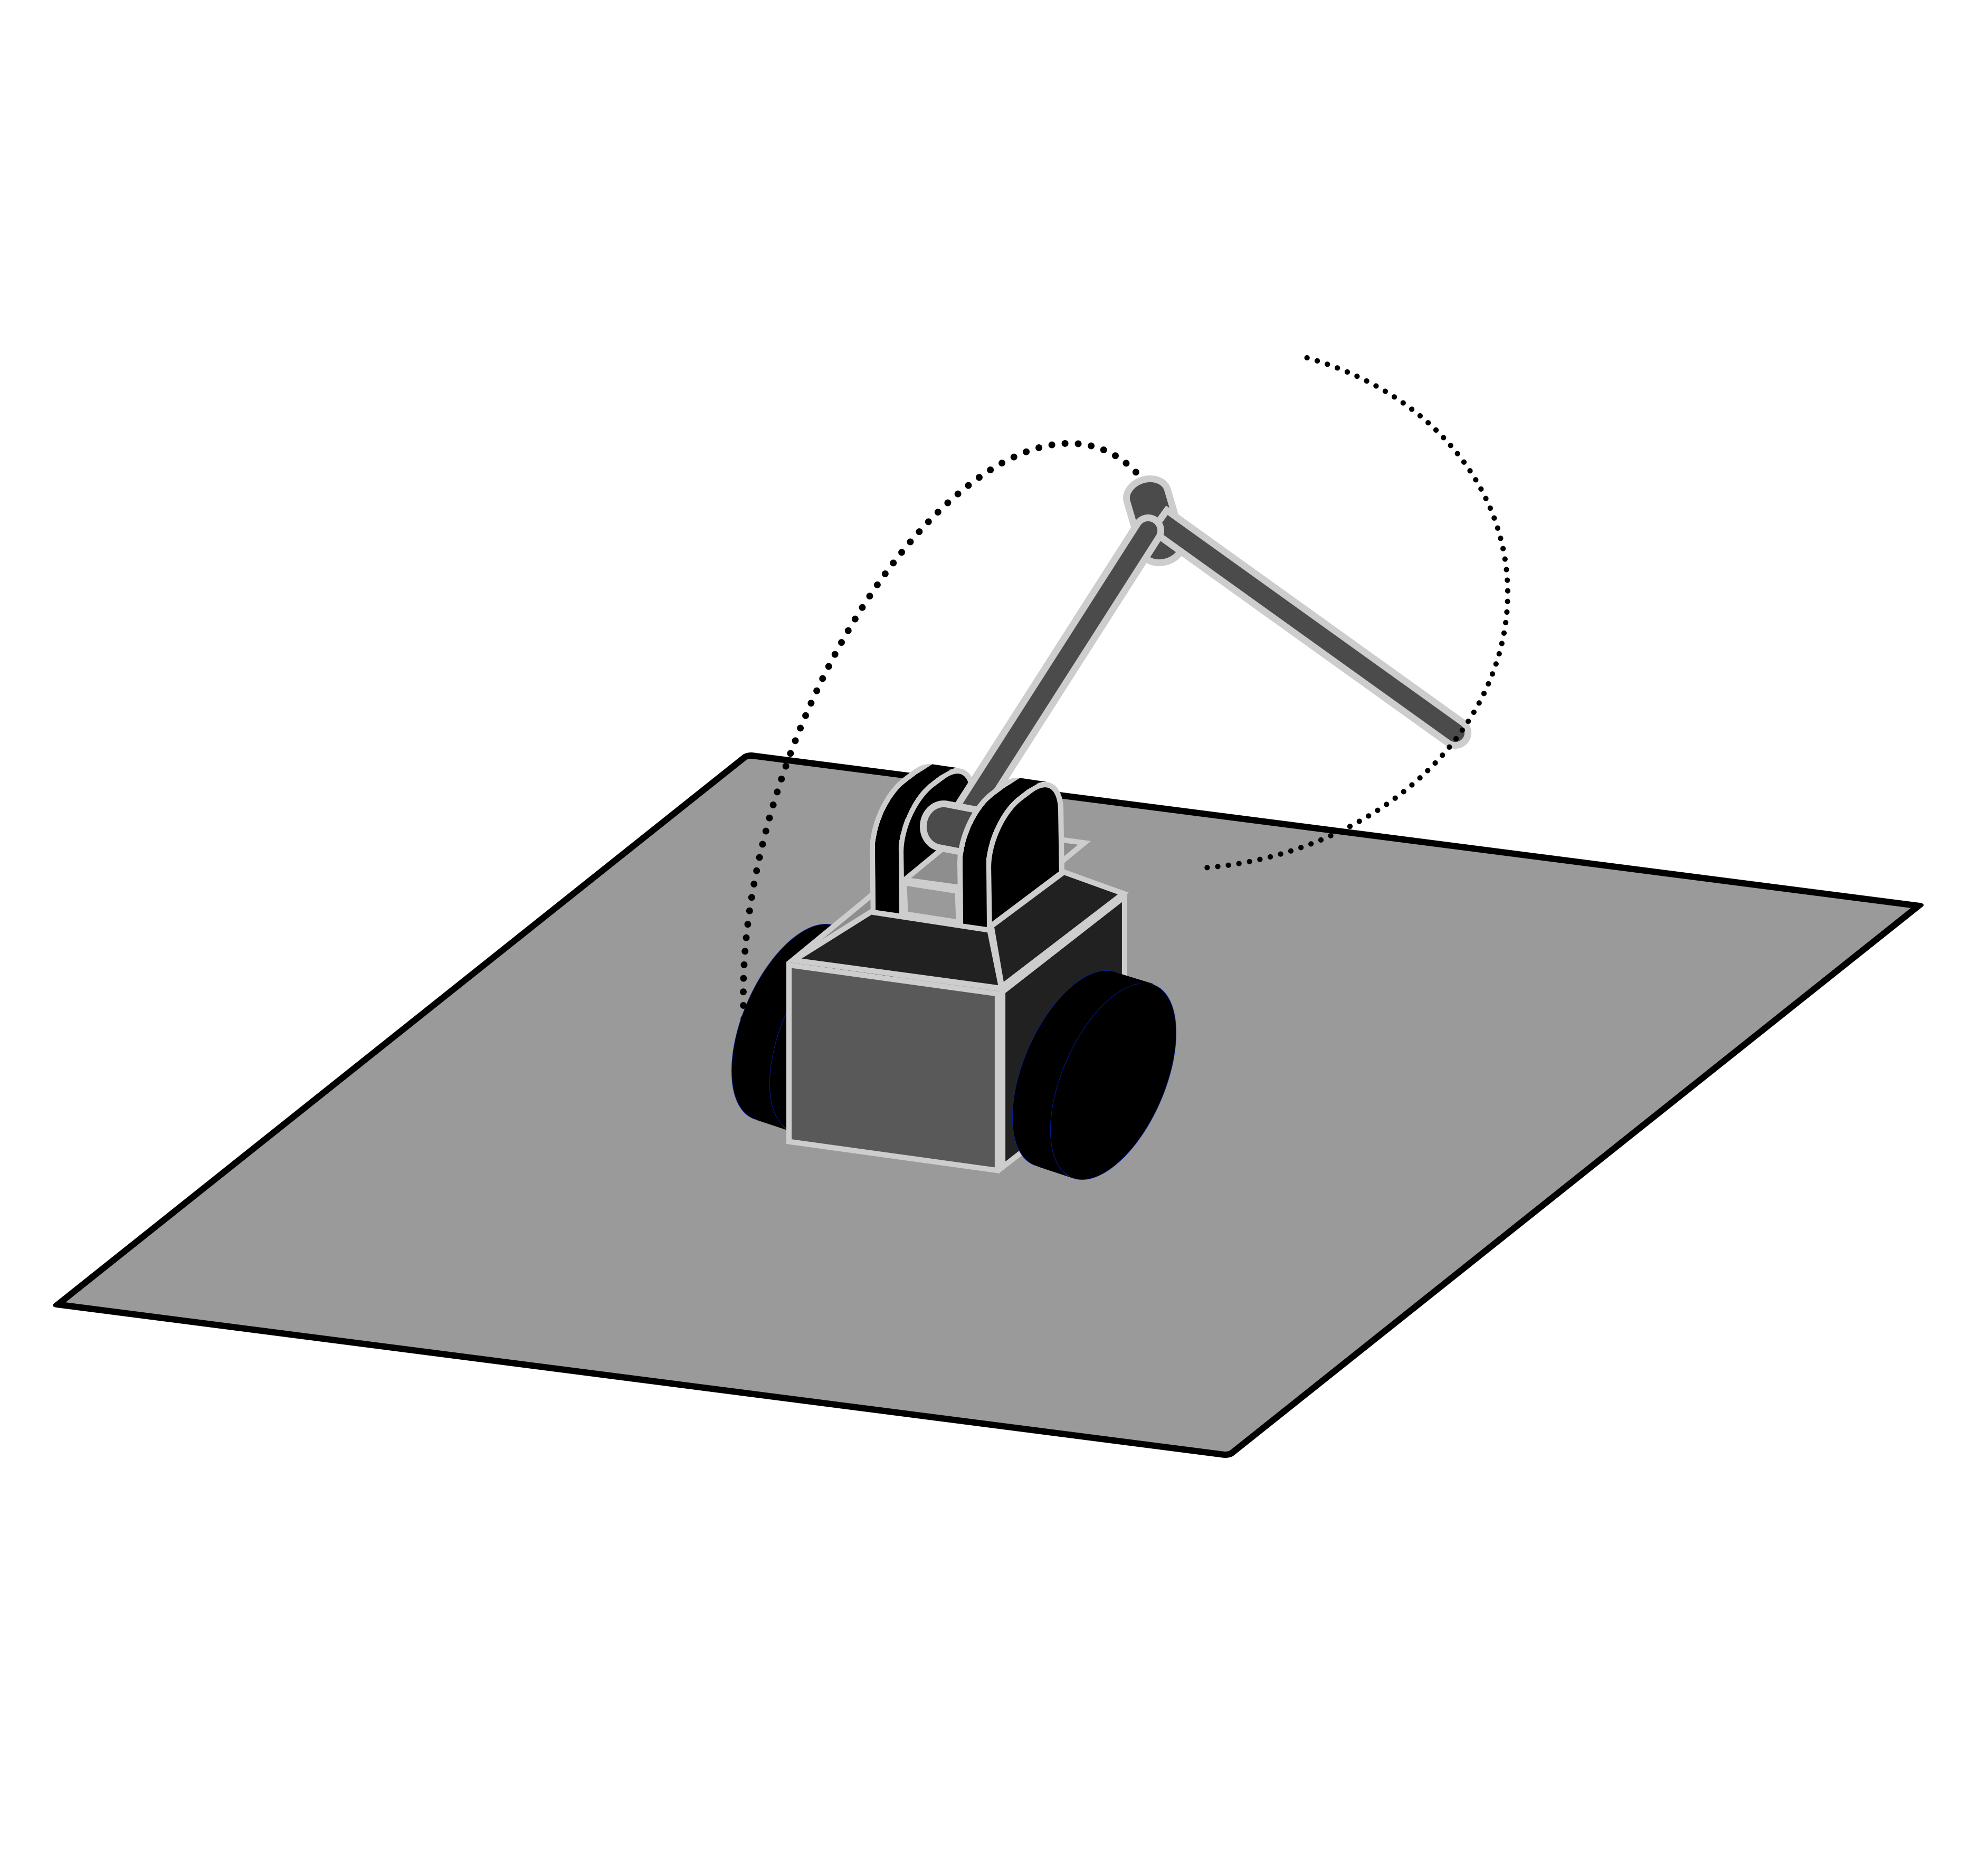
\includegraphics[width=0.4\textwidth]{vehicle-manipulator.jpg}
    \caption{Sample 2-link manipulator mounted on a Planar-joint base}
    \label{fig:planar}
\end{figure}

\section{Case Study: Spacecraft-Manipulator}

\begin{figure}
    \centering
    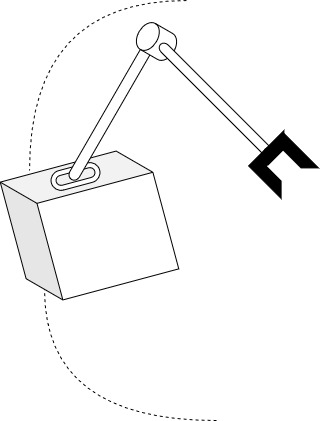
\includegraphics[width=0.2\textwidth]{Untitled Diagram(2).jpg}
    \caption{Sample 2-link manipulator mounted on a free-floating spacecraft base}
    \label{fig:my_label}
\end{figure}


\begin{comment}

The general Euler-Lagrange equations for $\mathcal{L}:TQ\rightarrow\R$ on a parameterzied ($q_b,\dot{q}_b,q_\mathfrak{m},\dot{q}_\mathfrak{m}$) configuration manifold $Q$, formulated as
\begin{equation*}
    \frac{d}{dt}(\frac{\partial \mathcal{L}}{\partial\dot{q}_{b_i}})-\frac{\partial \mathcal{L}}{\partial q_{b_i}}=\Gamma_{b_i} \quad q_{b_i} \in Q_b
\end{equation*}
\begin{equation}
    \frac{d}{dt}(\frac{\partial  \mathcal{L}}{\partial\dot{q}_i})-\frac{\partial \mathcal{L}}{\partial q_i}=\Gamma_i \quad q_i \in Q_\mathfrak{m}
\end{equation}
are equivalent to the Hamel's equations for a reduced lagrangian $l$ in a local principal bundle trivialization (see Appendix \ref{Appendix:geometric}).

\IEEEPARstart{W}{elcome} to the updated and simplified documentation to using the IEEEtran \LaTeX \ class file. The IEEE has examined hundreds of author submissions using this package to help formulate this easy to follow guide. We will cover the most commonly used elements of a journal article. For less common elements we will refer back to the ``IEEEtran\_HOWTO.pdf''.

This document applies to version 1.8b of IEEEtran. 

The IEEEtran template package contains the following example files: 
\begin{list}{}{}
\item{bare\_jrnl.tex}
\item{bare\_conf.tex}
\item{bare\_jrnl\_compsoc.tex}
\item{bare\_conf\_compsoc.tex}
\item{bare\_jrnl\_comsoc.tex}
\end{list}
These are ``bare bones" templates to quickly understand the document structure.  

It is assumed that the reader has a basic working knowledge of \LaTeX. Those who are new to \LaTeX \ are encouraged to read Tobias Oetiker's ``The Not So Short Introduction to \LaTeX '', available at: \url{http://tug.ctan.org/info/lshort/english/lshort.pdf} which provides an overview of working with \LaTeX.   

\section{The Design, Intent and \\ Limitations of the Templates}
\noindent The templates are intended to {\bf{approximate the final look and page length of the articles/papers}}. Therefore, {\bf{they are NOT intended to be the final produced work that is displayed in print or on IEEEXplore\textsuperscript{\textregistered}}}. They will help to give the authors an approximation of the number of pages that will be in the final version. The structure of the \LaTeX files, as designed, enable easy conversion to XML for the composition systems used by the IEEE's outsource vendors. The XML files are used to produce the final print/IEEEXplore\textsuperscript{\textregistered} pdf and then converted to HTML for IEEEXplore\textsuperscript{\textregistered}. Have you looked at your article/paper in the HTML version?

\section{\LaTeX \ Distributions: Where to Get Them}
\noindent IEEE recommends using the distribution from the \TeX User Group at \url{http://www.tug.org}. You can join TUG and obtain a DVD distribution or download for free  from the links provided on their website: \url{http://www.tug.org/texlive/}. The DVD includes distributions for Windows, Mac OS X and Linux operating systems.
 
\section{Where to get the IEEEtran Templates}
\noindent The {\bf{IEEE Template Selector}} will always have the most up-to-date versions of the \LaTeX\ and MSWord templates. Please see: \url{https://template-selector.ieee.org/} and follow the steps to find the correct template for your intended publication. Many publications use the IEEETran LaTeX templates, however, some publications have their own special templates. Many of these are  based on IEEEtran, but may have special instructions that vary slightly from those in this document.

\section{Where to get \LaTeX \ help - user groups}
\noindent The following on-line groups are very helpful to beginning and experienced \LaTeX\ users. A search through their archives can provide many answers to common questions.
\begin{list}{}{}
\item{\url{http://www.latex-community.org/}} 
\item{\url{https://tex.stackexchange.com/} }
\end{list}

\section{Document Class Options in IEEEtran}
\noindent At the beginning of your \LaTeX\ file you will need to establish what type of publication style you intend to use. The following list shows appropriate documentclass options for each of the types covered by IEEEtran.

\begin{list}{}{}
\item{Regular Journal Article}
\item{{\tt{$\backslash$documentclass[journal]{IEEEtran}}}}\\
\item{{Conference Paper}}
\item{{\tt{$\backslash$documentclass[conference]{IEEEtran}}}}\\
\item{Computer Society Journal Article}
\item{{\tt{$\backslash$documentclass[10pt,journal,compsoc]{IEEEtran}}}}\\
\item{Computer Society Conference Paper}
\item{{\tt{$\backslash$documentclass[conference,compsoc]{IEEEtran}}}}\\
\item{{Communications Society Journal Article}}
\item{{\tt{$\backslash$documentclass[journal,comsoc]{IEEEtran}}}}\\
\item{{Brief, Correspondence or Technote}}
\item{{\tt{$\backslash$documentclass[9pt,technote]{IEEEtran}}}}
\end{list}

There are other options available for each of these when submitting for peer review or other special requirements. IEEE recommends to compose your article in the base 2-column format to make sure all your equations, tables and graphics will fit the final 2-column format. Please refer to the document ``IEEEtran\_HOWTO.pdf'' for more information on settings for peer review submission if required by your EIC.

\section{How to Create Common Front Matter}
\noindent The following sections describe general coding for these common elements. Computer Society publications and Conferences may have their own special variations and will be noted below.
\subsection{Paper Title}
\noindent The title of your paper is coded as:

\begin{verbatim}
\title{The Title of Your Paper}
\end{verbatim}

\noindent Please try to avoid the use of math or chemical formulas in your title if possible.

\subsection{Author Names and Affiliations}
\noindent The author section should be coded as follows:
\begin{verbatim}
\author{Masahito Hayashi 
\IEEEmembership{Fellow, IEEE}, Masaki Owari
\thanks{M. Hayashi is with Graduate School 
of Mathematics, Nagoya University, Nagoya, 
Japan}
\thanks{M. Owari is with the Faculty of 
Informatics, Shizuoka University, 
Hamamatsu, Shizuoka, Japan.}
}
\end{verbatim}
Be sure to use the $\backslash$IEEEmembership command to identify IEEE membership status.
Please see the ``IEEEtran\_HOWTO.pdf'' for specific information on coding authors for Conferences and Computer Society publications. Note that the closing curly brace for the author group comes at the end of the thanks group. This will prevent you from creating a blank first page.

\subsection{Running Heads}
\noindent The running heads are declared by using the $\backslash${\tt{markboth}} command. There are two arguments to this command: the first contains the journal name information and the second contains the author names and paper title.
\begin{verbatim}
\markboth{Journal of Quantum Electronics, 
Vol. 1, No. 1, January 2021}
{Author1, Author2, 
\MakeLowercase{\textit{(et al.)}: 
Paper Title}
\end{verbatim}

\subsection{Copyright Line}
\noindent For Transactions and Journals papers, this is not necessary to use at the submission stage of your paper. The IEEE production process will add the appropriate copyright line. If you are writing a conference paper, please see the ``IEEEtran\_HOWTO.pdf'' for specific information on how to code "Publication ID Marks".

\subsection{Abstracts}
\noindent The abstract is the first element of a paper after the $\backslash${\tt{maketitle}} macro is invoked.  The coding is simply:
\begin{verbatim}
\begin{abstract}
Text of your abstract.
\end{abstract}
\end{verbatim}
Please try to avoid mathematical and chemical formulas in the abstract.

\subsection{Index Terms}
\noindent The index terms are used to help other researchers discover your paper. Each society may have it's own keyword set. Contact the EIC of your intended publication for this list.
\begin{verbatim}
\begin{IEEEkeywords}
Broad band networks, quality of service
\end{IEEEkeywords}
\end{verbatim}
\section{How to Create Common Body Elements}
\noindent The following sections describe common body text elements and how to code them.

\subsection{Initial Drop Cap Letter}
\noindent The first text paragraph uses a ``drop cap'' followed by the first word in ALL CAPS. This is accomplished by using the $\backslash${\tt{IEEEPARstart}} command as follows:
\begin{verbatim}
\IEEEPARstart{T}{his} is the first paragraph 
of your paper. . .
\end{verbatim}

\subsection{Sections and Subsections}
\noindent Section headings use standard \LaTeX\ commands: $\backslash${\tt{section}}, $\backslash${\tt{subsection}} and $\backslash${\tt{subsubsection}}. Numbering is handled automatically for you and varies according to type of publication. It is common to not indent the first paragraph following a section head by using $\backslash${\tt{noindent}} as follows:
\begin{verbatim}
\section{Section Head}
\noindent The text of your paragraph . . .
\end{verbatim}

\subsection{Citations to the Bibliography}
\noindent The coding for the citations are made with the \LaTeX\ $\backslash${\tt{cite}} command. This will produce individual bracketed reference numbers in the IEEE style. At the top of your \LaTeX\ file you should include:
\begin{verbatim}
\usepackage{cite}
\end{verbatim}
For a single citation code as follows:
\begin{verbatim}
see \cite{ams}
\end{verbatim}
This will display as: see \cite{ams}\\

For multiple citations code as follows:
\begin{verbatim}
\cite{ams,oxford,lacomp}
\end{verbatim}

This will display as \cite{ams,oxford,lacomp}

\subsection{Figures}
\noindent Figures are coded with the standard \LaTeX\ commands as follows:
\begin{verbatim}
\begin{figure}[!t]
\centering
\includegraphics[width=2.5in]{fig1}
\caption{This is the caption for one fig.}
\label{fig1}
\end{figure}
\end{verbatim}
The [!t] argument enables floats to the top of the page to follow IEEE style. Make sure you include:
\begin{verbatim}
\usepackage{graphicx}
\end{verbatim}
 
\noindent at the top of your \LaTeX file with the other package declarations. 

To cross-reference your figures in the text use the following code example:
\begin{verbatim}
See figure \ref{fig1} ...
\end{verbatim}
This will produce:\\
See figure \ref{fig1} . . .

\begin{figure}[!t]
\centering
\includegraphics[width=2.5in]{fig1}
\caption{This is the caption for one fig.}
\label{fig1}
\end{figure}

\subsection{Tables}
\noindent Tables should be coded with the standard \LaTeX\ coding. The following example shows a simple table.


\begin{verbatim}
\begin{table}
\begin{center}
\caption{Filter design equations  ...}
\label{tab1}
\begin{tabular}{| c | c | c |}
\hline
Order & Arbitrary coefficients & 
coefficients\\
of filter & $e_\mathfrak{m}$ &   $b_{ij}$ \\
\hline
1& $b_{ij}=\hat{e}.\hat{\beta_{ij}}$, 
& $b_{00}=0$\\
\hline
2&$\beta_{22}=(~1,-1,-1,~~1,~~1,~~1)$ &\\ 
\hline
3& $b_{ij}=\hat{e}.\hat{\beta_{ij}}$, 
& $b_{00}=0$,\\
\hline 
\end{tabular}
\end{center}
\end{table}
\end{verbatim}
To reference the table in the text, code as follows:
\begin{verbatim}Table~\ref{tab1} lists the closed-form...\end{verbatim}
to produce:

Table~\ref{tab1} lists the closed-form . . .


%moved here for pagination purposes
\begin{table}
\begin{center}
\caption{A Simple Table Example.}
\label{tab1}
\begin{tabular}{| c | c | c |}
\hline
Order & Arbitrary coefficients & coefficients\\
of filter & $e_\mathfrak{m}$ &   $b_{ij}$ \\
\hline
1& $b_{ij}=\hat{e}.\hat{\beta_{ij}}$, & $b_{00}=0$\\
\hline
2&$\beta_{22}=(~1,-1,-1,~~1,~~1,~~1)$ &\\ 
\hline
3& $b_{ij}=\hat{e}.\hat{\beta_{ij}}$, & $b_{00}=0$,\\
\hline 
\end{tabular}
\end{center}
\end{table}


\subsection{Lists}
\noindent In this section, we will consider three types of lists: simple unnumbered, numbered and bulleted. There have been numerous options added to IEEEtran to enhance the creation of lists. If your lists are more complex than those shown below, please refer to the  ``IEEEtran\_HOWTO.pdf'' for additional options.\\

\noindent{\bf A plain  unnumbered list}

\begin{list}{}{}
\item{bare\_jrnl.tex}
\item{bare\_conf.tex}
\item{bare\_jrnl\_compsoc.tex}
\item{bare\_conf\_compsoc.tex}
\item{bare\_jrnl\_comsoc.tex}
\end{list}

\noindent coded as:
\begin{verbatim}
\begin{list}{}{}
\item{bare\_jrnl.tex}
\item{bare\_conf.tex}
\item{bare\_jrnl\_compsoc.tex}
\item{bare\_conf\_compsoc.tex}
\item{bare\_jrnl\_comsoc.tex}
\end{list}
\end{verbatim}
\noindent{\bf A simple numbered list}

\begin{enumerate}
\item{bare\_jrnl.tex}
\item{bare\_conf.tex}
\item{bare\_jrnl\_compsoc.tex}
\item{bare\_conf\_compsoc.tex}
\item{bare\_jrnl\_comsoc.tex}
\end{enumerate}
\noindent coded as: 
\begin{verbatim}
\begin{enumerate}
\item{bare\_jrnl.tex}
\item{bare\_conf.tex}
\item{bare\_jrnl\_compsoc.tex}
\item{bare\_conf\_compsoc.tex}
\item{bare\_jrnl\_comsoc.tex}
\end{enumerate}
\end{verbatim}

\noindent{\bf A simple bulleted list}

\begin{itemize}
\item{bare\_jrnl.tex}
\item{bare\_conf.tex}
\item{bare\_jrnl\_compsoc.tex}
\item{bare\_conf\_compsoc.tex}
\item{bare\_jrnl\_comsoc.tex}
\end{itemize}

\noindent coded as:

\begin{verbatim}
\begin{itemize}
\item{bare\_jrnl.tex}
\item{bare\_conf.tex}
\item{bare\_jrnl\_compsoc.tex}
\item{bare\_conf\_compsoc.tex}
\item{bare\_jrnl\_comsoc.tex}
\end{itemize}
\end{verbatim}


\subsection{Other Elements}
\noindent For other less common elements such as Algorithms, Theorems and Proofs, and Floating Structures such as page-wide tables, figures or equations, please refer to the ``IEEEtran\_HOWTO.pdf'' section on ``Double Column Floats.''


\section{How to Create Common Back Matter Elements}
\noindent The following sections demonstrate common back matter elements such as Acknowledgments, Bibliographies, Appendicies and Author Biographies.

\subsection{Acknowledgments}
\noindent This should be a simple paragraph before the bibliography to thank those individuals and institutions who have supported your work on this article.

\begin{verbatim}
\section{Acknowledgments}
\noindent Text describing those who 
supported your paper.
\end{verbatim}

\subsection{Bibliographies}
\noindent {\bf{References Simplified:}} A simple way of composing references is to use the $\backslash${\tt{bibitem}} macro to define the beginning of a reference as in the following examples:\\


\noindent [6] H. Sira-Ramirez. ``On the sliding mode control of nonlinear systems,'' \textit{Systems \& Control Letters}, vol. 19, pp. 303--312, 1992.

\noindent coded as:
\begin{verbatim}
\bibitem{Sira3}
H. Sira-Ramirez. ``On the sliding mode 
control of nonlinear systems,'' 
\textit{Systems \& Control Letters}, 
vol. 19, pp. 303--312, 1992.
\end{verbatim}

\noindent [7] A. Levant.``Exact differentiation of signals with unbounded higher derivatives,''  in \textit{Proceedings of the 45th IEEE Conference on Decision and Control}, San Diego, California, USA, pp. 5585--5590, 2006.

\noindent coded as:
\begin{verbatim}\bibitem{Levant}
A. Levant. ``Exact differentiation of 
signals with unbounded higher 
derivatives,''  in \textit{Proceedings 
of the 45th IEEE Conference on 
Decision and Control}, San Diego, 
California, USA, pp. 5585--5590, 2006.
\end{verbatim}


\noindent [8] M. Fliess, C. Join, and H. Sira-Ramirez. ``Non-linear estimation is easy,'' \textit{International Journal of Modelling, Identification and Control}, vol. 4, no. 1, pp. 12--27, 2008.

\noindent coded as:
\begin{verbatim}
\bibitem{Cedric}
M. Fliess, C. Join, and H. Sira-Ramirez. 
``Non-linear estimation is easy,'' 
\textit{International Journal of Modelling, 
Identification and Control}, vol. 4, 
no. 1, pp. 12--27, 2008.
\end{verbatim}

\noindent [9] R. Ortega, A. Astolfi, G. Bastin, and H. Rodriguez. ``Stabilization of food-chain systems using a port-controlled Hamiltonian description,'' in \textit{Proceedings of the American Control Conference}, Chicago, Illinois, USA, pp. 2245--2249, 2000.

\noindent coded as:
\begin{verbatim}
\bibitem{Ortega}
R. Ortega, A. Astolfi, G. Bastin, and H. 
Rodriguez. ``Stabilization of food-chain 
systems using a port-controlled Hamiltonian 
description,'' in \textit{Proceedings of the 
American Control Conference}, Chicago, 
Illinois, USA, pp. 2245--2249, 2000.
\end{verbatim}

\subsection{Accented Characters in References}
\noindent When using accented characters in references, please use the standard LaTeX coding for accents. {\bf{Do not use math coding for character accents}}. For example:
\begin{verbatim}
\'e, \"o, \`a, \~e 
\end{verbatim}
will produce: \'e, \"o, \`a, \~e 


\subsection{Use of BibTeX}
\noindent If you wish to use BibTeX, please see the documentation that accompanies the IEEEtran Bibliography package.

\subsection{Biographies and Author Photos}
\noindent Authors may have options to include their photo or not. Photos should be a bit-map graphic (.tif or .jpg) and sized to fit in the space allowed. Please see the coding samples below:
\begin{verbatim}
\begin{IEEEbiographynophoto}{Jane Doe}
Biography text here without a photo.
\end{IEEEbiographynophoto}
\end{verbatim}
or a biography with a photo

\begin{verbatim}
\begin{IEEEbiography}[{\includegraphics
[width=1in,height=1.25in,clip,
keepaspectratio]{fig1.png}}]
{IEEE Publications Technology Team} 
In this paragraph you can place 
your educational, professional background 
and research and other interests.
\end{IEEEbiography}
\end{verbatim}

Please see the end of this document to see the output of these coding examples.



\section{Mathematical Typography \\ and Why It Matters}

\noindent Typographical conventions for mathematical formulas have been developed to {\bf provide uniformity and clarity of presentation across mathematical texts}. This enables the readers of those texts to both understand the author's ideas and to grasp new concepts quickly. While software such as \LaTeX \ and MathType\textsuperscript{\textregistered} can produce aesthetically pleasing math when used properly, it is also very easy to misuse the software, potentially resulting in incorrect math display.

IEEE aims to provide authors with the proper guidance on mathematical typesetting style and assist them in writing the best possible article.

As such, IEEE has assembled a set of examples of good and bad mathematical typesetting. You will see how various issues are dealt with. The following publications have been referenced in preparing this material:

\begin{list}{}{}
\item{\emph{Mathematics into Type}, published by the American Mathematical Society}
\item{\emph{The Printing of Mathematics}, published by Oxford University Press}
\item{\emph{The \LaTeX Companion}, by F. Mittelbach and M. Goossens}
\item{\emph{More Math into LaTeX}, by G. Gr\"atzer}
\item{AMS-StyleGuide-online.pdf, published by the American Mathematical Society}
\end{list}

Further examples can be seen at \url{http://journals.ieeeauthorcenter.ieee.org/wp-content/uploads/sites/7/IEEE-Math-Typesetting-Guide.pdf}

\subsection{Display Equations}
\noindent A simple display equation example shown below uses the ``equation'' environment. To number the equations, use the $\backslash${\tt{label}} macro to create an identifier for the equation. LaTeX will automatically number the equation for you.
\begin{equation}
\label{deqn_ex1}
x = \sum_{i=0}^{n} 2{i} Q.
\end{equation}

\noindent is coded as follows:
\begin{verbatim}
\begin{equation}
\label{deqn_ex1}
x = \sum_{i=0}^{n} 2{i} Q.
\end{equation}
\end{verbatim}

To reference this equation in the text use the $\backslash${\tt{ref}} macro. 
Please see (\ref{deqn_ex1})\\
\noindent is coded as follows:
\begin{verbatim}
Please see (\ref{deqn_ex1})\end{verbatim}

\subsection{Equation Numbering}
\noindent {\bf{Consecutive Numbering:}} Equations within an article are numbered consecutively from the beginning of the
article to the end, i.e., (1), (2), (3), (4), (5), etc. Do not use roman numerals or section numbers for equation numbering.\\

\noindent {\bf{Appendix Equations:}} The continuation of consecutively numbered equations is best in the Appendix, but numbering
 as (A1), (A2), etc., is permissible.\\

\noindent {\bf{Hyphens and Periods}}: Hyphens and periods should not be used in equation numbers, i.e., use (1a) rather than
(1-a) and (2a) rather than (2.a) for sub-equations. This should be consistent throughout the article.

\subsection{Multi-line equations and alignment}
\noindent Here we show several examples of multi-line equations and proper alignments.

\noindent {\bf{A single equation that must break over multiple lines due to length with no specific alignment.}}
\begin{multline}
\text{The first line of this example}\\
\text{The second line of this example}\\
\text{The third line of this example}
\end{multline}

\noindent is coded as:
\begin{verbatim}
\begin{multline}
\text{The first line of this example}\\
\text{The second line of this example}\\
\text{The third line of this example}
\end{multline}
\end{verbatim}

\noindent {\bf{A single equation with multiple lines aligned at the = signs}}
\begin{align}
a &= c+d \\
b &= e+f
\end{align}
\noindent is coded as:
\begin{verbatim}
\begin{align}
a &= c+d \\
b &= e+f
\end{align}
\end{verbatim}

The {\tt{align}} environment can align on multiple  points as shown in the following example:
\begin{align}
x &= y & X & =Y & a &=bc\\
x' &= y' & X' &=Y' &a' &=bz
\end{align}
\noindent is coded as:
\begin{verbatim}
\begin{align}
x &= y & X & =Y & a &=bc\\
x' &= y' & X' &=Y' &a' &=bz
\end{align}
\end{verbatim}





\subsection{Subnumbering}
\noindent The amsmath package provides a {\tt{subequations}} environment to facilitate subnumbering. An example:

\begin{subequations}\label{eq:2}
\begin{align}
f&=g \label{eq:2A}\\
f' &=g' \label{eq:2B}\\
\mathcal{L}f &= \mathcal{L}g \label{eq:2c}
\end{align}
\end{subequations}

\noindent is coded as:
\begin{verbatim}
\begin{subequations}\label{eq:2}
\begin{align}
f&=g \label{eq:2A}\\
f' &=g' \label{eq:2B}\\
\mathcal{L}f &= \mathcal{L}g \label{eq:2c}
\end{align}
\end{subequations}

\end{verbatim}

\subsection{Matrices}
\noindent There are several useful matrix environments that can save you some keystrokes. See the example coding below and the output.

\noindent {\bf{A simple matrix:}}
\begin{equation}
\begin{matrix}  0 &  1 \\ 
1 &  0 \end{matrix}
\end{equation}
is coded as:
\begin{verbatim}
\begin{equation}
\begin{matrix}  0 &  1 \\ 
1 &  0 \end{matrix}
\end{equation}
\end{verbatim}

\noindent {\bf{A matrix with parenthesis}}
\begin{equation}
\begin{pmatrix} 0 & -i \\
 i &  0 \end{pmatrix}
\end{equation}
is coded as:
\begin{verbatim}
\begin{equation}
\begin{pmatrix} 0 & -i \\
 i &  0 \end{pmatrix}
\end{equation}
\end{verbatim}

\noindent {\bf{A matrix with square brackets}}
\begin{equation}
\begin{bmatrix} 0 & -1 \\ 
1 &  0 \end{bmatrix}
\end{equation}
is coded as:
\begin{verbatim}
\begin{equation}
\begin{bmatrix} 0 & -1 \\ 
1 &  0 \end{bmatrix}
\end{equation}
\end{verbatim}

\noindent {\bf{A matrix with curly braces}}
\begin{equation}
\begin{Bmatrix} 1 &  0 \\ 
0 & -1 \end{Bmatrix}
\end{equation}
is coded as:
\begin{verbatim}
\begin{equation}
\begin{Bmatrix} 1 &  0 \\ 
0 & -1 \end{Bmatrix}
\end{equation}\end{verbatim}

\noindent {\bf{A matrix with single verticals}}
\begin{equation}
\begin{vmatrix} a &  b \\ 
c &  d \end{vmatrix}
\end{equation}
is coded as:
\begin{verbatim}
\begin{equation}
\begin{vmatrix} a &  b \\ 
c &  d \end{vmatrix}
\end{equation}\end{verbatim}

\noindent {\bf{A matrix with double verticals}}
\begin{equation}
\begin{Vmatrix} i &  0 \\ 
0 & -i \end{Vmatrix}
\end{equation}
is coded as:
\begin{verbatim}
\begin{equation}
\begin{Vmatrix} i &  0 \\ 
0 & -i \end{Vmatrix}
\end{equation}\end{verbatim}

\subsection{Arrays}
\noindent The {\tt{array}} environment allows you some options for matrix-like equations. You will have to manually key the fences, but you'll have options for alignment of the columns and for setting horizontal and vertical rules. The argument to {\tt{array}} controls alignment and placement of vertical rules.

A simple array
\begin{equation}
\left(
\begin{array}{cccc}
a+b+c & uv & x-y & 27\\
a+b & u+v & z & 134
\end{array}\right)
\end{equation}
is coded as:
\begin{verbatim}
\begin{equation}
\left(
\begin{array}{cccc}
a+b+c & uv & x-y & 27\\
a+b & u+v & z & 134
\end{array} \right)
\end{equation}
\end{verbatim}

A slight variation on this to better align the numbers in the last column
\begin{equation}
\left(
\begin{array}{cccr}
a+b+c & uv & x-y & 27\\
a+b & u+v & z & 134
\end{array}\right)
\end{equation}
is coded as:
\begin{verbatim}
\begin{equation}
\left(
\begin{array}{cccr}
a+b+c & uv & x-y & 27\\
a+b & u+v & z & 134
\end{array} \right)
\end{equation}
\end{verbatim}

An array with vertical and horizontal rules
\begin{equation}
\left( \begin{array}{c|c|c|r}
a+b+c & uv & x-y & 27\\ \hline
a+b & u+v & z & 134
\end{array}\right)
\end{equation}
is coded as:
\begin{verbatim}
\begin{equation}
\left(
\begin{array}{c|c|c|r}
a+b+c & uv & x-y & 27\\
a+b & u+v & z & 134
\end{array} \right)
\end{equation}
\end{verbatim}
Note the argument now has the pipe "$\vert$" included to indicate the placement of the vertical rules.


\subsection{Cases Structures}
\noindent Many times we find cases coded using the wrong environment, i.e., {\tt{array}}. Using the {\tt{cases}} environment will save keystrokes (from not having to type the $\backslash${\tt{left}}$\backslash${\tt{lbrace}}) and automatically provide the correct column alignment.
\begin{equation*}
{z_\mathfrak{m}(t)} = \begin{cases}
1,&{\text{if}}\ {\beta }_\mathfrak{m}(t) \\ 
{0,}&{\text{otherwise.}} 
\end{cases}
\end{equation*}
\noindent is coded as follows:
\begin{verbatim}
\begin{equation*}
{z_\mathfrak{m}(t)} = 
\begin{cases}
1,&{\text{if}}\ {\beta }_\mathfrak{m}(t),\\ 
{0,}&{\text{otherwise.}} 
\end{cases}
\end{equation*}
\end{verbatim}
\noindent Note that the ``\&'' is used to mark the tabular alignment. This is important to get  proper column alignment. Do not use $\backslash${\tt{quad}} or other fixed spaces to try and align the columns. Also, note the use of the $\backslash${\tt{text}} macro for text elements such as ``if'' and ``otherwise''.

\subsection{Function Formatting in Equations}
In many cases there is an easy way to properly format most common functions. Use of the $\backslash$ in front of the function name will in most cases, provide the correct formatting. When this does not work, the following example provides a solution using the $\backslash${\tt{text}} macro.

\begin{equation*} 
  d_{R}^{KM} = \underset {d_{l}^{KM}} {\text{arg min}} \{ d_{1}^{KM},\ldots,d_{6}^{KM}\}.
\end{equation*}

\noindent is coded as follows:
\begin{verbatim}
\begin{equation*} 
 d_{R}^{KM} = \underset {d_{l}^{KM}} 
 {\text{arg min}} \{ d_{1}^{KM},
 \ldots,d_{6}^{KM}\}.
\end{equation*}
\end{verbatim}

\subsection{ Text Acronyms inside equations}
\noindent This example shows where the acronym ``MSE" is coded using $\backslash${\tt{text\{\}}} to match how it appears in the text.

\begin{equation*}
 \text{MSE} = \frac {1}{n}\sum _{i=1}^{n}(Y_{i} - \hat {Y_{i}})^{2}
\end{equation*}

\begin{verbatim}
\begin{equation*}
 \text{MSE} = \frac {1}{n}\sum _{i=1}^{n}
(Y_{i} - \hat {Y_{i}})^{2}
\end{equation*}
\end{verbatim}

\subsection{Obsolete Coding}
\noindent Avoid the use of outdated environments, such as {\tt{eqnarray}} and \$\$ math delimiters, for display equations. The \$\$ display math delimiters are left over from PlainTeX and should not be used in \LaTeX, ever. Poor vertical spacing will result.
\subsection{Use Appropriate Delimiters for Display Equations}
\noindent Some improper mathematical coding advice has been given in various YouTube\textsuperscript{TM} videos on how to write scholarly articles, so please follow these good examples:\\

For {\bf{single-line unnumbered display equations}}, please use the following delimiters: 
\begin{verbatim}\[ . . . \] or \end{verbatim} 
\begin{verbatim}\begin{equation*} . . . \end{equation*}\end{verbatim}
Note that the * in the environment name turns off equation numbering.\\

For {\bf{multiline unnumbered display equations}} that have alignment requirements, please use the following delimiters: 
\begin{verbatim}
\begin{align*} . . . \end{align*}
\end{verbatim}

For {\bf{single-line numbered display equations}}, please use the following delimiters: 
\begin{verbatim}
\begin{equation} . . . \end{equation}
\end{verbatim}

For {\bf{multiline numbered display equations}}, please use the following delimiters: 
\begin{verbatim}
\begin{align} . . . \end{align}
\end{verbatim}

\section{LaTeX Package Suggestions}
\noindent Immediately after your documenttype declaration at the top of your \LaTeX\ file is the place where you should declare any packages that are being used. The following packages were used in the production of this document.
\begin{verbatim}
\usepackage{amsmath,amsfonts}
\usepackage{algorithmic}
\usepackage{array}
\usepackage[caption=false,font=normalsize,
   labelfont=sf,textfont=sf]{subfig}
\u00sepackage{textcomp}
\usepackage{stfloats}
\usepackage{url}
\usepackage{verbatim}
\usepackage{graphicx}
\usepackage{balance}
\end{verbatim}

\section{Additional Advice}

Please use ``soft'' (e.g., \verb|\eqref{Eq}|) or \verb|(\ref{Eq})|
cross references instead of ``hard'' references (e.g., \verb|(1)|).
That will make it possible to combine sections, add equations, or
change the order of figures or citations without having to go through
the file line by line.

Please note that the \verb|{subequations}| environment in {\LaTeX}
will increment the main equation counter even when there are no
equation numbers displayed. If you forget that, you might write an
article in which the equation numbers skip from (17) to (20), causing
the copy editors to wonder if you've discovered a new method of
counting.

{\BibTeX} does not work by magic. It doesn't get the bibliographic
data from thin air but from .bib files. If you use {\BibTeX} to produce a
bibliography you must send the .bib files. 

{\LaTeX} can't read your mind. If you assign the same label to a
subsubsection and a table, you might find that Table I has been cross
referenced as Table IV-B3. 

{\LaTeX} does not have precognitive abilities. If you put a
\verb|\label| command before the command that updates the counter it's
supposed to be using, the label will pick up the last counter to be
cross referenced instead. In particular, a \verb|\label| command
should not go before the caption of a figure or a table.

Please do not use \verb|\nonumber| or \verb|\notag| inside the
\verb|{array}| environment. It will not stop equation numbers inside
\verb|{array}| (there won't be any anyway) and it might stop a wanted
equation number in the surrounding equation.

\balance

\section{A Final Checklist}
\begin{enumerate}{}{}
\item{Make sure that your equations are numbered sequentially and there are no equation numbers missing or duplicated. Avoid hyphens and periods in your equation numbering. Stay with IEEE style, i.e., (1), (2), (3) or for sub-equations (1a), (1b). For equations in the appendix (A1), (A2), etc.}. 
\item{Are your equations properly formatted? Text, functions, alignment points in cases and arrays, etc. }
\item{Make sure all graphics are included.}
\item{Make sure your references are included either in your main LaTeX file or a separate .bib file if calling the external file.}
\end{enumerate}


\end{comment}

\bibliographystyle{ieeetr}
\bibliography{references}


\end{document}


